\documentclass[class=NCU_thesis, crop=false]{standalone}
\begin{document}

\chapter{實驗設計與結果}

\section{資料集}
本研究使用為合作醫院所提供之資料集,為心臟範圍之電腦斷層掃描影像,
電腦斷層掃描設備輸出之原始影像數值為HU值。資料集分別有三大類資料:
\begin{enumerate}
\item 已標記之有顯影劑增強影像,共21組,
每一組影像為256張,大小為512*512,
其針對冠狀動脈血管分成四類進行標記,分別為RCA、LM、LAD、LCx。
運用於訓練以有顯影劑增強電腦斷層影像進行冠狀動脈分割之模型,
以及利用風格轉換模型產生虛擬的無顯影劑增強電腦斷層掃描影像,
做為無顯影劑增強冠狀動脈分割模型的擴增資料。
\item 已標記之無顯影劑增強影像,共10組,
每一組影像為64張,大小為512*512,
其將所有冠狀動脈視為一類進行標記,
運用於訓練對無顯影劑增強電腦斷層影像進行冠狀動脈分割之模型。
\item 未標記之同一個案之有顯影劑增強影像與無顯影劑增強影像,共45組,
其中28組影像為2*256張、 16組影像為2*224張、1組影像為2*192張,大小皆為512*512,
運用於訓練將有顯影劑增強影像轉換為無顯影劑增強影像之模型。
\end{enumerate}

%資料集統整如\cref{table:table-dataset}。
%\begin{table}[h]
%    \centering
%    \caption{有顯影劑增強之電腦斷層掃描分割結果}
%    \label{table:table-dataset}
%    \begin{tabularx}{\textwidth}{|c|c|c|c|c|}
%    \hline
%    資料名稱 & 冠狀動脈標記 & 原始影像大小 & 資料數量 & 用途 \\
%    \hline
%    已標記之有顯影劑增強影像 & 有,分四類血管 & (512, 512, 256) & 21組 
%    & 1. 訓練有顯影劑之冠狀動脈分割模型 2. 透過風格轉換模型,轉換為無顯影劑增強之擴充影像 \\
%    \hline
%    已標記之無顯影劑增強影像 & 有,全部冠狀動脈視為一類 & (512, 512, 256) & 10組 
%    & 訓練無顯影劑之冠狀動脈分割模型 \\
%    \hline
%    未標記之同一個案之有顯影劑增強影像與無顯影劑增強影像 & 無 & (512, 512, 256) & 45組 
%    & 訓練風格轉換模型,將有顯影劑影像轉換為虛擬無顯影劑影像 \\
%    \hline
%    \end{tabularx}
%\end{table}

\section{有顯影劑增強影像之冠狀動脈分割}

本研究利用21組已標註冠狀動脈的有顯影劑增強之電腦斷層影像,
訓練以有顯影劑增強之電腦斷層影像進行冠狀動脈分割之3D U-Net模型,
由於實驗樣本數較少,以K-fold交叉驗證方式進行實驗,
其中18組做為訓練資料,3組做為測試資料,
總共分為7個Fold進行實驗。

模型輸入為前處理後的三維影像,
訓練資料如\cref{fig:fig-dataset-contrast-input-example}所示,
其中\cref{fig:fig-dataset-contrast-192-S}為電腦斷層掃描單切的影像,
每一組壓縮後的資料一共會有192切影像,
並可以藉由堆疊組成三維的影像,
以透過不同方向如\cref{fig:fig-dataset-contrast-192-R}
以及\cref{fig:fig-dataset-contrast-192-P}來進行觀察。
\cref{fig:fig-dataset-contrast-192-S}、
\cref{fig:fig-dataset-contrast-192-R}、
\cref{fig:fig-dataset-contrast-192-P}
中有顏色部分為人工標記的冠狀動脈位置,
淺藍色為RCA、綠色為LM、深藍色為LCx、黃色為LAD,為3D U-Net之預期輸出,
\cref{fig:fig-dataset-contrast-192-label}為冠狀動脈標記以之三維影像呈現的結果。
\begin{figure}[!hbt]
    %\captionsetup[subfigure]{labelformat=empty} % 完全隱藏圖號
    \centering
    \subcaptionbox
        {由下往上方向
        \label{fig:fig-dataset-contrast-192-S}}
        {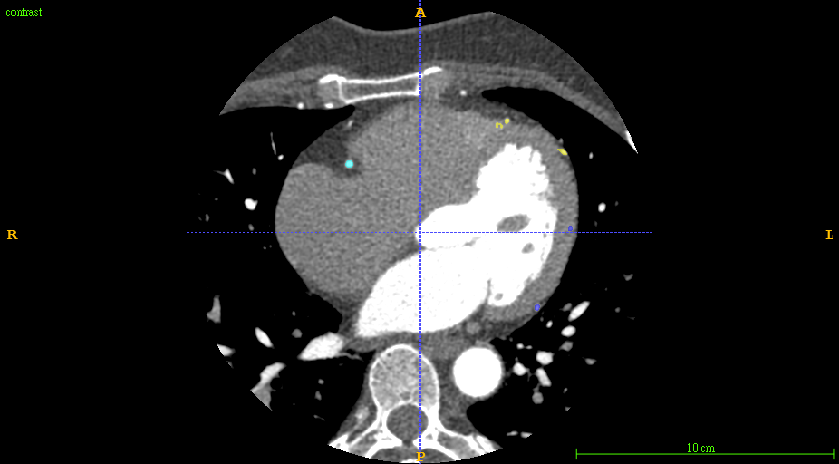
\includegraphics[width=0.475\linewidth]{fig-dataset-contrast-192-S.jpg}}
    ~
    \subcaptionbox
        {由左往右方向
        \label{fig:fig-dataset-contrast-192-R}}
        {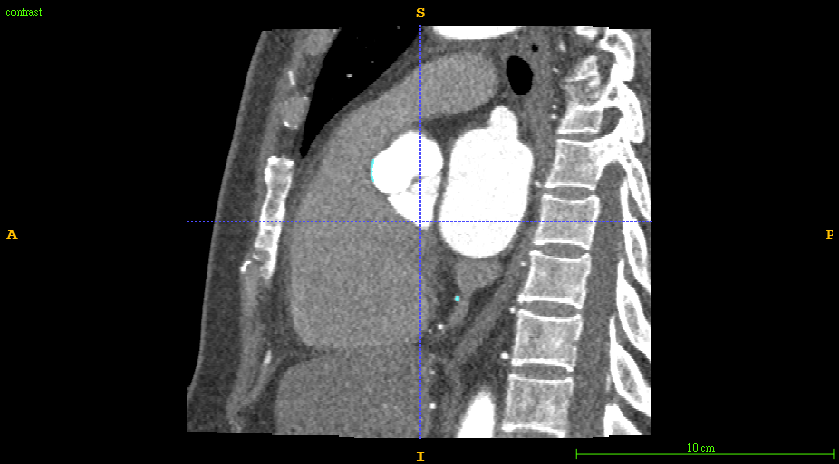
\includegraphics[width=0.475\linewidth]{fig-dataset-contrast-192-R.jpg}}
    \vspace{\baselineskip} % 分隔上下列
    \subcaptionbox
        {由前往後方向
        \label{fig:fig-dataset-contrast-192-P}}
        {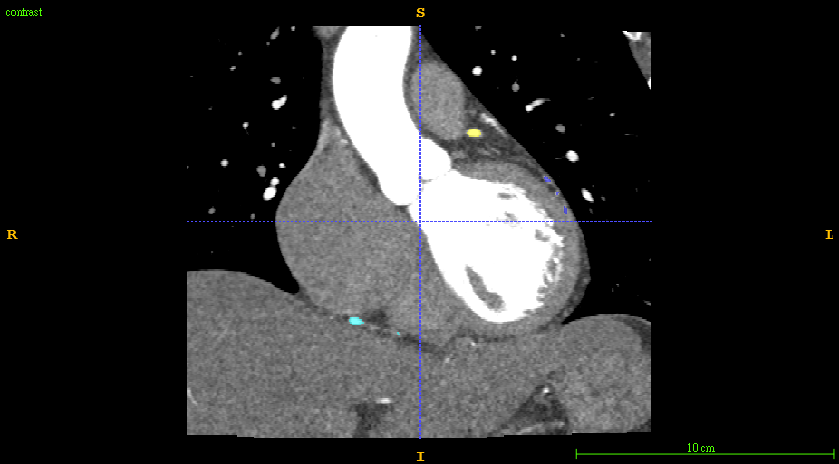
\includegraphics[width=0.475\linewidth]{fig-dataset-contrast-192-P.jpg}}
    ~
    \subcaptionbox
        {以三維影像呈現之冠狀動脈標註
        \label{fig:fig-dataset-contrast-192-label}}
        {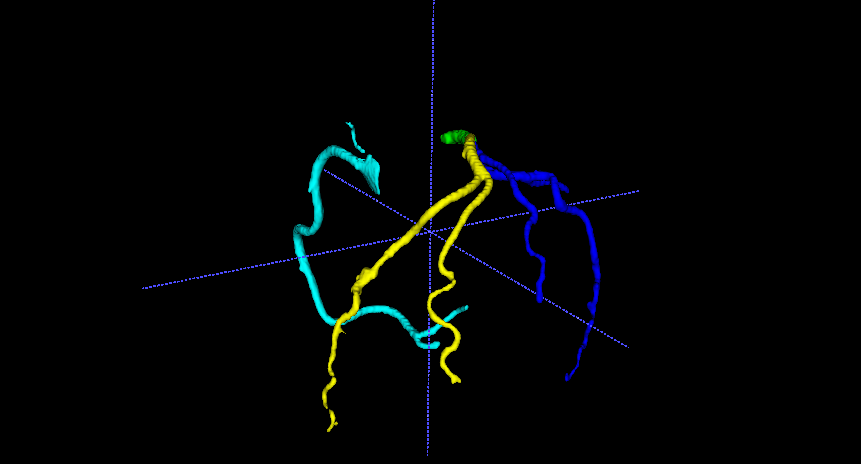
\includegraphics[width=0.475\linewidth]{fig-dataset-contrast-192-label.jpg}}
    \caption{模型訓練資料範例-有顯影劑增強}
    \label{fig:fig-dataset-contrast-input-example}
\end{figure}

模型訓練所使用目標函數為骰子損失函數(Dice Loss),函式為\cref{eqn:dice-loss},
各分類冠狀動脈將分別計算各分類的目標函數。

\begin{equation}
\label{eqn:dice-loss}
Loss = 1-\frac{2|X\cap Y|}{|X|+|Y|} 
\end{equation}

模型結果以骰子係數(Dice Coefficient)進行評估,
其函式為\cref{eqn:dice-coefficient},
骰子係數之值愈高,則代表模型分割結果與人工標記結果重合部分越多,反之則愈少。
\begin{equation}
\label{eqn:dice-coefficient}
Dice Coefficient = \frac{2|X\cap Y|}{|X|+|Y|} 
\end{equation}

訓練完成的模型以7-Fold交叉驗證對於測試資料集之結果如\cref{table:table-contrast-7-fold-result},
\cref{table:table-contrast-7-fold-result}列出各類血管分類的Dice Coefficient,
以及將所有血管視為一類的Dice Coefficient結果。

\begin{table}[h]
    \centering
    \caption{有顯影劑增強之電腦斷層掃描7-Fold交叉驗證結果}
    \label{table:table-contrast-7-fold-result}
    \begin{tabular}{cccccc}
    \hline
    \multirow{2}{*}{Fold} & \multicolumn{5}{c}{Dice Coefficient} \\
    \cline{2-6}
    & All & RCA & LM & LAD & LCx \\
    \hline
    1 & 0.7942 & 0.7918 & 0.7156 & 0.6868 & 0.7559 \\
    2 & 0.7674 & 0.7934 & 0.4106 & 0.6718 & 0.5660 \\
    3 & 0.7941 & 0.7838 & 0.7214 & 0.6642 & 0.6066 \\
    4 & 0.7859 & 0.7954 & 0.6040 & 0.7237 & 0.7064 \\
    5 & 0.7650 & 0.6837 & 0.6911 & 0.6811 & 0.7169 \\
    6 & 0.7644 & 0.7806 & 0.5654 & 0.6077 & 0.6233 \\
    7 & 0.8368 & 0.8248 & 0.7608 & 0.7984 & 0.7414 \\
    \hline
    Average & \textbf{0.7868} & 0.7791 & 0.6384 & 0.6905 & 0.6738 \\
    \hline
    \end{tabular}
\end{table}

結果顯示,
本研究所實驗之3D U-Net模型對於測試資料集,
以全部冠狀動脈分割在7-Fold交叉驗證中平均能達到Dice Coefficient 0.7868的結果,
影響結果Dice Coefficient的狀況有分割錯誤以及分類錯誤,
分割錯誤為未分割出標記中所包含的血管或是分割出的結果不在標記中,
\cref{fig:fig-sample-contrast-result-bad-segmentation-error}為一個分割錯誤的範例,
可以看到\cref{fig:fig-sample-contrast-result-bad-segmentation-error-prediction}之模型分割結果較
\cref{fig:fig-sample-contrast-result-bad-segmentation-error-label}之人工標記缺少一些部分,
而分類錯誤則是分割出之結果是冠狀動脈,但血管分類並不正確,
\cref{fig:fig-sample-contrast-result-bad-classification-error-label}為一個分類錯誤的範例,
部分分類錯誤的情形也導致\cref{table:table-contrast-7-fold-result}個別血管的結果會較整體血管的Dice Coefficient來的低,
血管分類中表現較好者為RCA,
由於RCA與LM、LAD、LCx位置距離較遠,推測是其在分割與分類上結果較好的原因,
血管分類中較差且不同實驗差異較大的為LM,
推測原因為LM本身體積較小且LM又會分支為LAD、LCx,
因此在分支交界處常發生分類錯誤的情形,
而由於其體積較小,當分類錯誤發生時會較大幅度地影響其結果之Dice Coefficient。

\begin{figure}[!hbt]
    %\captionsetup[subfigure]{labelformat=empty} % 完全隱藏圖號
    \centering
    \subcaptionbox
        {人工標記結果
        \label{fig:fig-sample-contrast-result-bad-segmentation-error-label}}
        {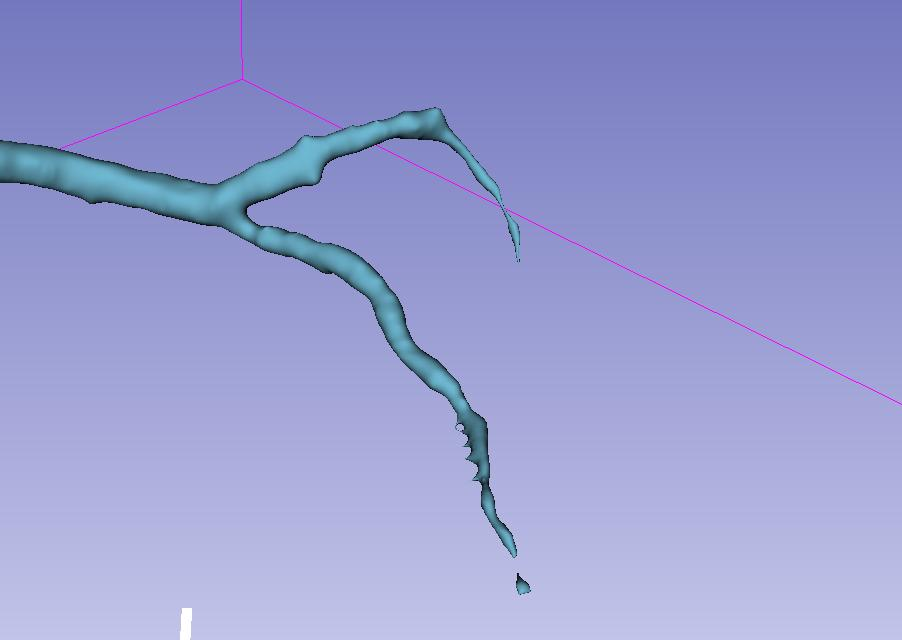
\includegraphics[width=0.475\linewidth]{fig-sample-contrast-result-bad-segmentation-error-label.jpg}}
    ~
    \subcaptionbox
        {模型輸出結果
        \label{fig:fig-sample-contrast-result-bad-segmentation-error-prediction}}
        {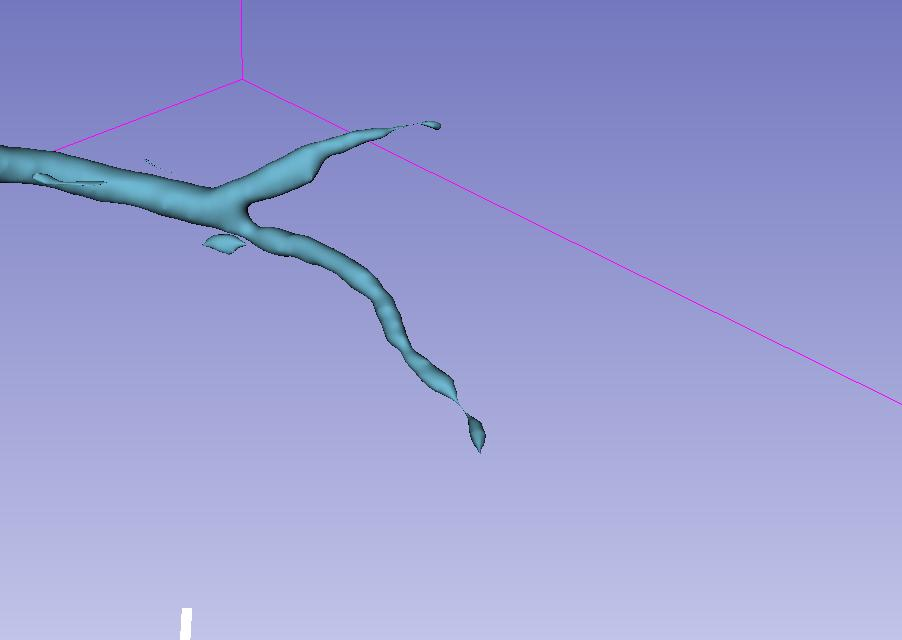
\includegraphics[width=0.475\linewidth]{fig-sample-contrast-result-bad-segmentation-error-prediction.jpg}}
    \caption{模型分割錯誤範例}
    \label{fig:fig-sample-contrast-result-bad-segmentation-error}
\end{figure}

\begin{figure}[!hbt]
    %\captionsetup[subfigure]{labelformat=empty} % 完全隱藏圖號
    \centering
    \subcaptionbox
        {人工標記結果
        \label{fig:fig-sample-contrast-result-bad-classification-error-label}}
        {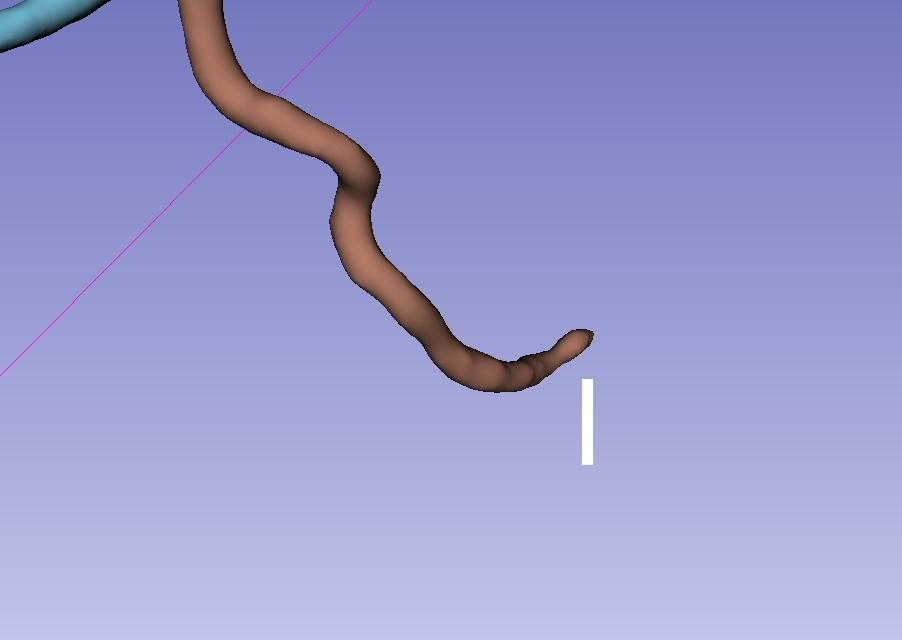
\includegraphics[width=0.475\linewidth]{fig-sample-contrast-result-bad-classification-error-label.jpg}}
    ~
    \subcaptionbox
        {模型輸出結果
        \label{fig:fig-sample-contrast-result-bad-classification-error-prediction}}
        {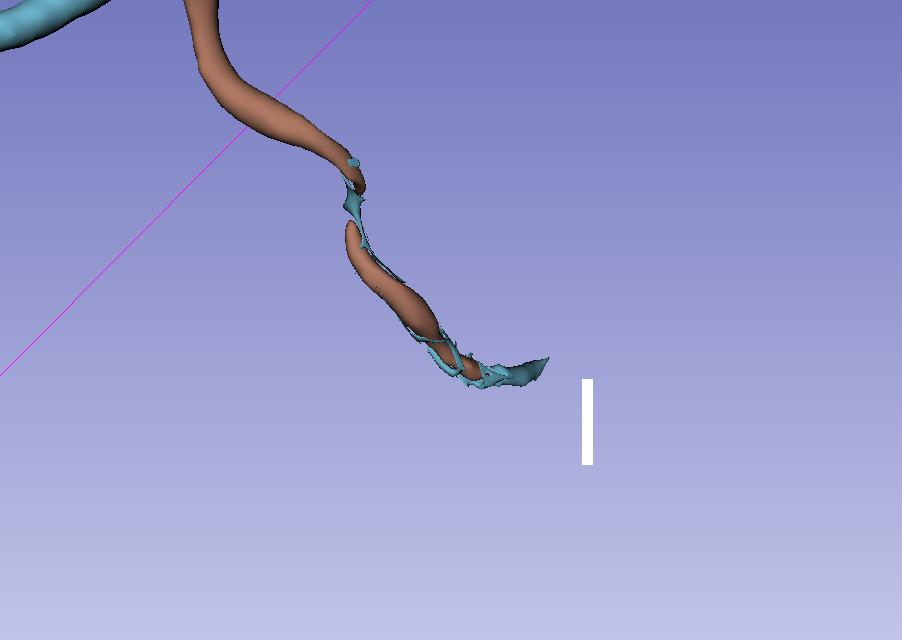
\includegraphics[width=0.475\linewidth]{fig-sample-contrast-result-bad-classification-error-prediction.jpg}}
    \caption{模型分類錯誤範例}
    \label{fig:fig-sample-contrast-result-bad-classification-error}
\end{figure}

與其他相關研究的結果比較如\cref{table:table-contrast-result-compare-others},
以Dice Coefficient數值來說,
本研究相較於Moeskops等人~\cite{moeskopsDeepLearningMultitask2016}與Huang等人~\cite{huangCoronaryArterySegmentation2018}之結果較好,
但是並不如Chen等人~\cite{chenCoronaryArterySegmentation2019}之結果,
此部分會因為本研究使用的資料為合作醫院所提供,
與其他研究的結果直接進行比較會有一些偏差,不一定為絕對的較好或較差,
然而本研究沒有使用額外的前處理資料如Huang等人~\cite{huangCoronaryArterySegmentation2018}所使用的中心線
以及Chen等人~\cite{chenCoronaryArterySegmentation2019}所使用的血管增強處理方法,
卻能達到相近甚至較好的結果,
這部分認為是因為本研究沒有將原始資料以Patch的方式切割,
而是將影像壓縮至192*192*192大小以完整影像進行訓練的原因,
因此在不進行後處理的情況下,本研究的冠狀動脈結果能有較少的雜訊。

\begin{table}[h]
    \centering
    \caption{有顯影劑增強之電腦斷層掃描分割結果與其他研究比較}
    \label{table:table-contrast-result-compare-others}
    \begin{tabular}{cccc}
    \hline
    本研究 & Moeskops等人~\cite{moeskopsDeepLearningMultitask2016} & Huang等人~\cite{huangCoronaryArterySegmentation2018} & Chen等人~\cite{chenCoronaryArterySegmentation2019} \\
    \hline
    \textbf{0.7868} & 0.65 & 0.7755 & 0.8060 \\
    \hline
    \end{tabular}
\end{table}

\cref{fig:fig-sample-contrast-result-good-1}為一模型較佳之輸出結果範例,
可以觀察到在輸出結果中冠狀動脈大致皆有被正確的分割與分類,
然而在較末端與較小的血管尚有一些分割錯誤,
如\cref{fig:fig-sample-contrast-result-good-1-label}中人工標記之藍色與中黃色之部分血管在\cref{fig:fig-sample-contrast-result-good-1-prediction}中模型輸出結果中並未被正確分割出來,
然而模型也有額外分割出人工標記中未標記到的部分,如\cref{fig:fig-sample-contrast-result-good-1-prediction}中棕色的最下方,
顯示模型對於冠狀動脈分割的能力有一定的推廣性。


\begin{figure}[!hbt]
    %\captionsetup[subfigure]{labelformat=empty} % 完全隱藏圖號
    \centering
    \subcaptionbox
        {人工標記結果
        \label{fig:fig-sample-contrast-result-good-1-label}}
        {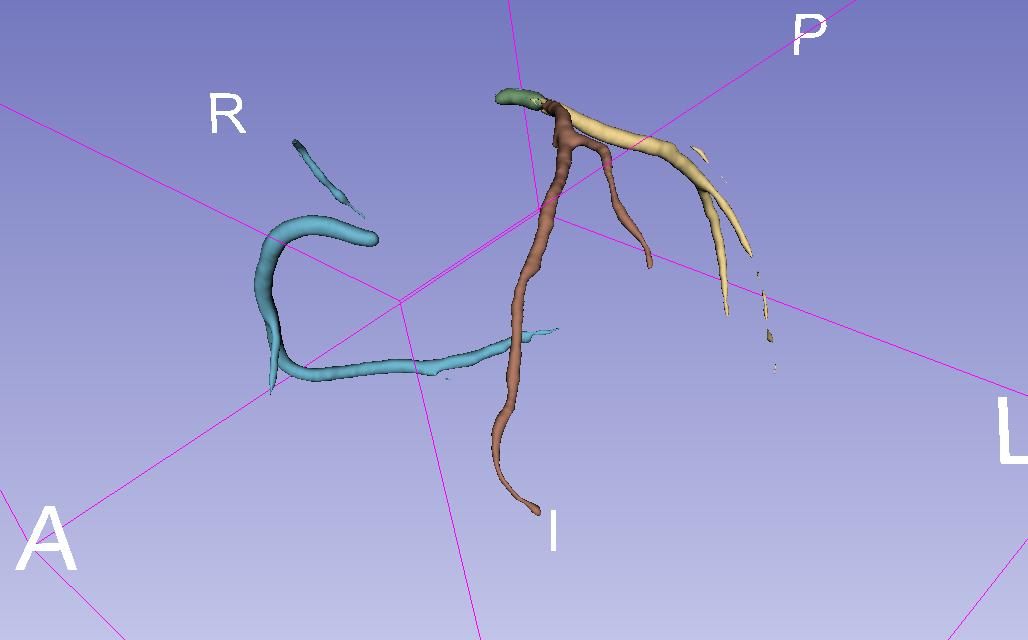
\includegraphics[width=0.475\linewidth]{fig-sample-contrast-result-good-1-label.jpg}}
    ~
    \subcaptionbox
        {模型輸出結果
        \label{fig:fig-sample-contrast-result-good-1-prediction}}
        {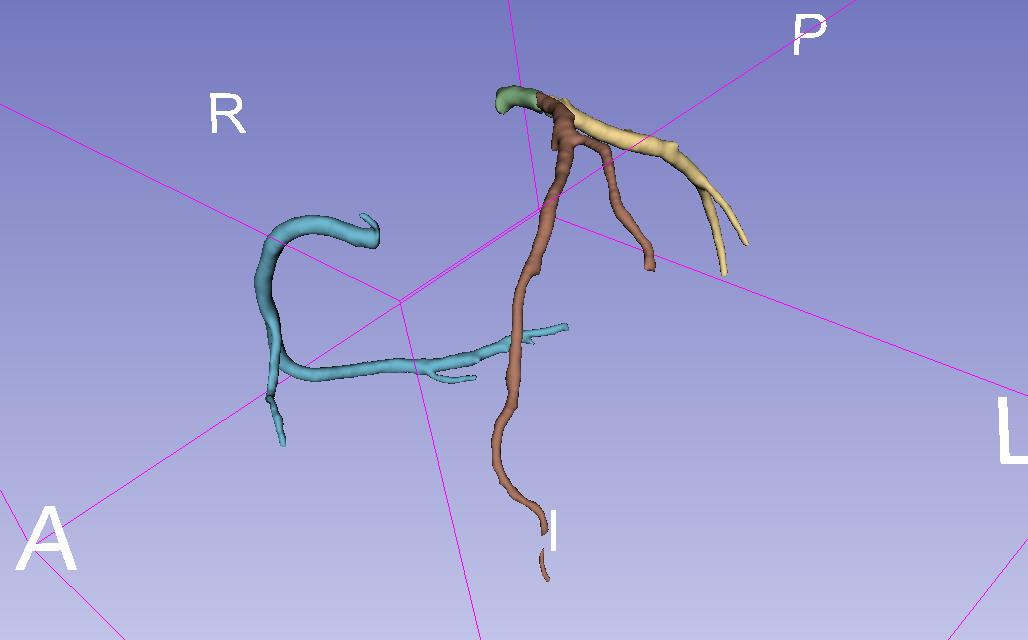
\includegraphics[width=0.475\linewidth]{fig-sample-contrast-result-good-1-prediction.jpg}}
    \caption{有顯影劑增強之電腦斷層掃描分割較佳結果範例}
    \label{fig:fig-sample-contrast-result-good-1}
\end{figure}


\cref{fig:fig-sample-contrast-result-bad-1}為一模型較差之輸出結果範例,
可以觀察到在輸出結果中冠狀動脈大致皆有被正確的分割與分類,
然而此範例有較多之分割錯誤,
如\cref{fig:fig-sample-contrast-result-bad-1-prediction}中多出之藍色以及棕色分割,
以及棕色與黃色部分有較多未分割出來的狀況,
此外也有一些分類錯誤的情形,
不過整體仍然能正確的分割出大部分的冠狀動脈。

\begin{figure}[!hbt]
    %\captionsetup[subfigure]{labelformat=empty} % 完全隱藏圖號
    \centering
    \subcaptionbox
        {人工標記結果
        \label{fig:fig-sample-contrast-result-bad-1-label}}
        {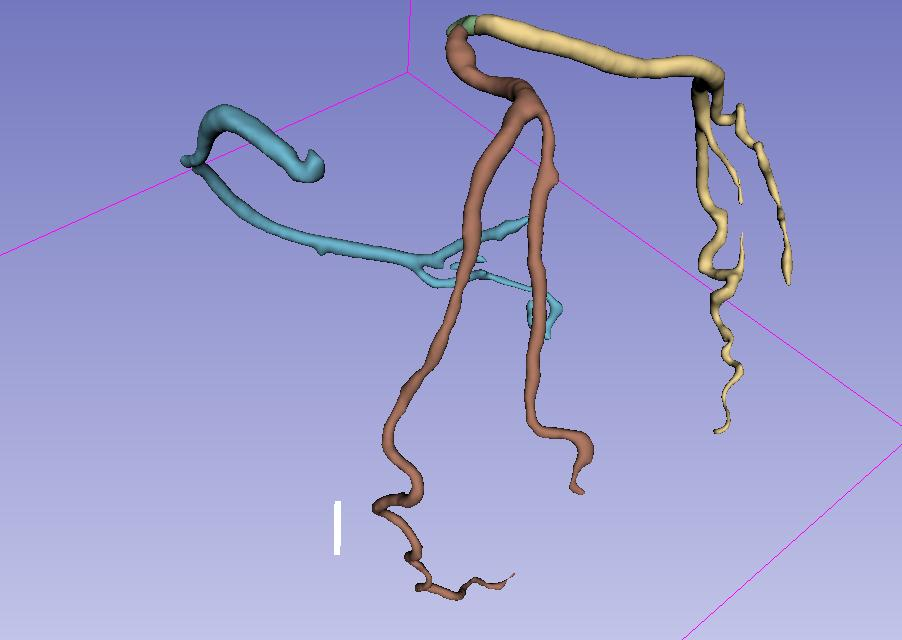
\includegraphics[width=0.475\linewidth]{fig-sample-contrast-result-bad-1-label.jpg}}
    ~
    \subcaptionbox
        {模型輸出結果
        \label{fig:fig-sample-contrast-result-bad-1-prediction}}
        {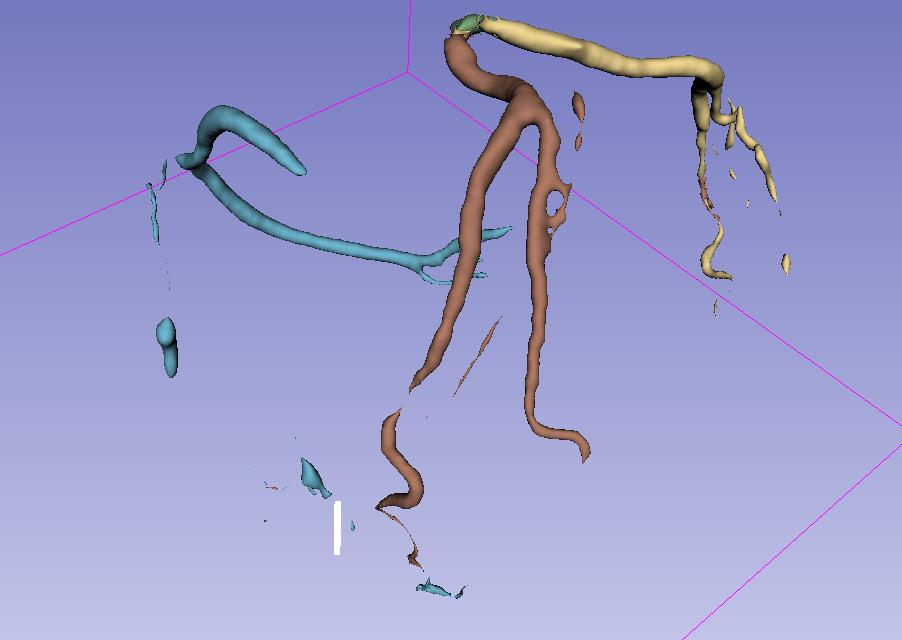
\includegraphics[width=0.475\linewidth]{fig-sample-contrast-result-bad-1-prediction.jpg}}
    \caption{有顯影劑增強之電腦斷層掃描分割較差結果範例}
    \label{fig:fig-sample-contrast-result-bad-1}
\end{figure}
% 
% \begin{figure}[!ht]
%     \centering
%     \setkeys{Gin}{width=\linewidth}
%     \begin{subfigure}{0.45\textwidth}
%         \caption*{人工標註結果}
%     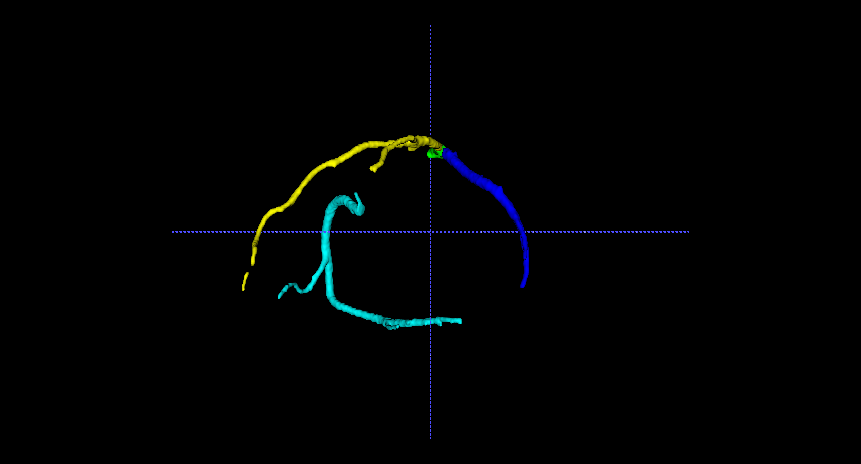
\includegraphics{fig-sample-contrast-result-1-label}\\[3pt]
%     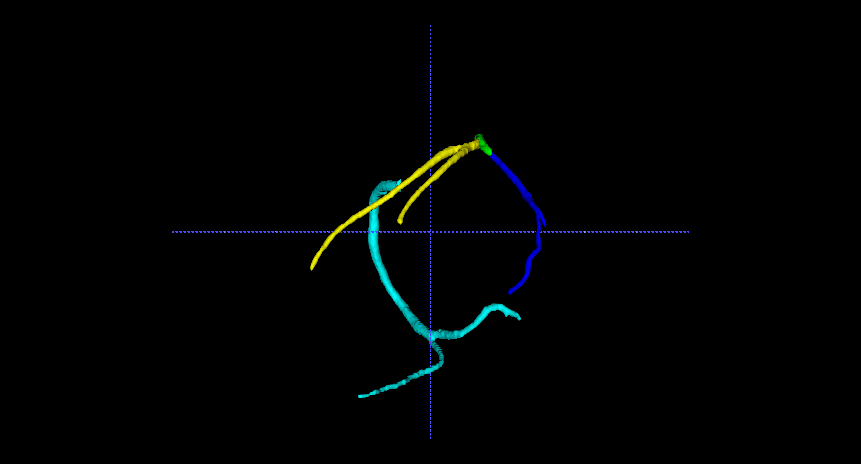
\includegraphics{fig-sample-contrast-result-2-label}
%     \end{subfigure}
%     \hfil
%     \begin{subfigure}{0.45\linewidth}
%         \caption*{模型輸出結果}
%     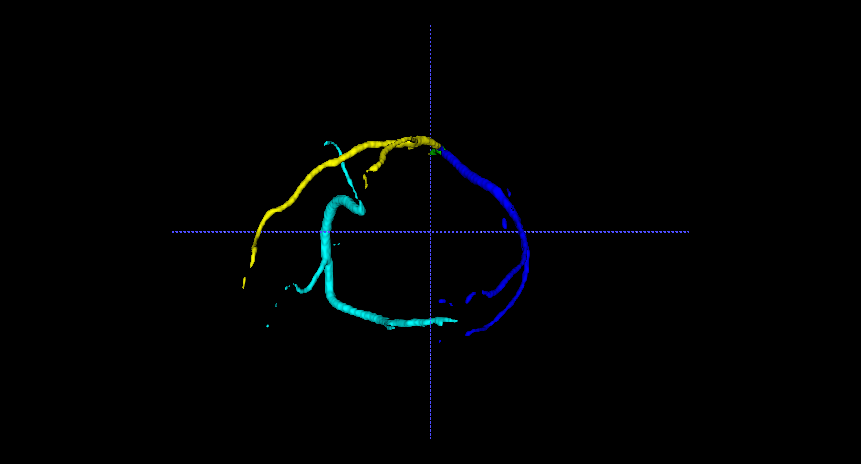
\includegraphics{fig-sample-contrast-result-1-prediction}\\[3pt]
%     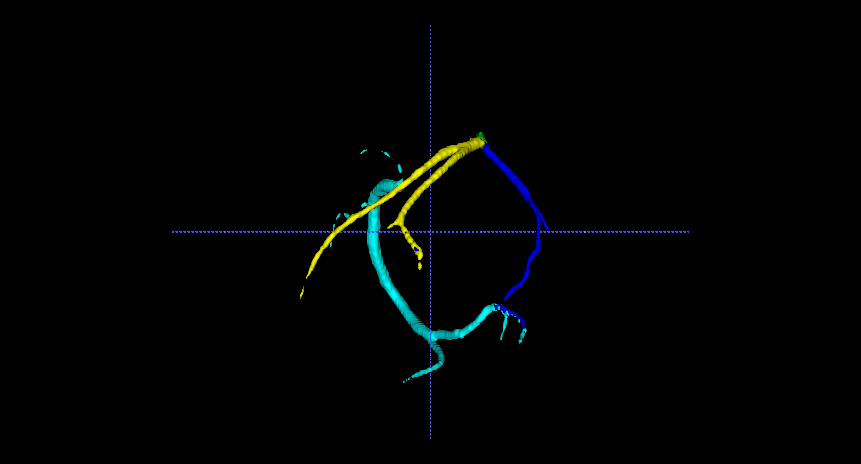
\includegraphics{fig-sample-contrast-result-2-prediction}
%     \end{subfigure}
%         \caption{有顯影劑增強之電腦斷層掃描分割結果}
%     \label{fig:fig-sample-contrast-result}
% \end{figure}
% 

\section{電腦斷層掃描影像風格轉換}
本研究利用45組擁有無注射顯影劑以及有注射顯影劑的受檢者資料,
訓練將電腦斷層影像由有顯影劑增強轉換為無顯影劑增強之CycleGAN模型,
模型輸入資料為單張2D電腦斷層掃描影像,包含有顯影劑增強以及無顯影劑增強之影像,
總計共有10944張2D電腦斷層影像,其中9792張做為訓練資料、1152張做為測試資料。

訓練結果最好的CycleGAN模型對於測試資料結果如\cref{fig:fig-sample-gan},
\cref{fig:fig-sample-gan}中最左邊為CycleGAN輸入之原始有顯影劑增強之電腦斷層影像,
中間為CycleGAN轉換後的虛擬無顯影劑增強電腦斷層影像,
右邊為同一受檢者於相同位置的真實無顯影劑增強電腦斷層影像。
\begin{figure}[!ht]
    \centering
    \setkeys{Gin}{width=\linewidth}
    \begin{subfigure}{0.3\textwidth}
        \caption*{真實有顯影劑增強影像}
    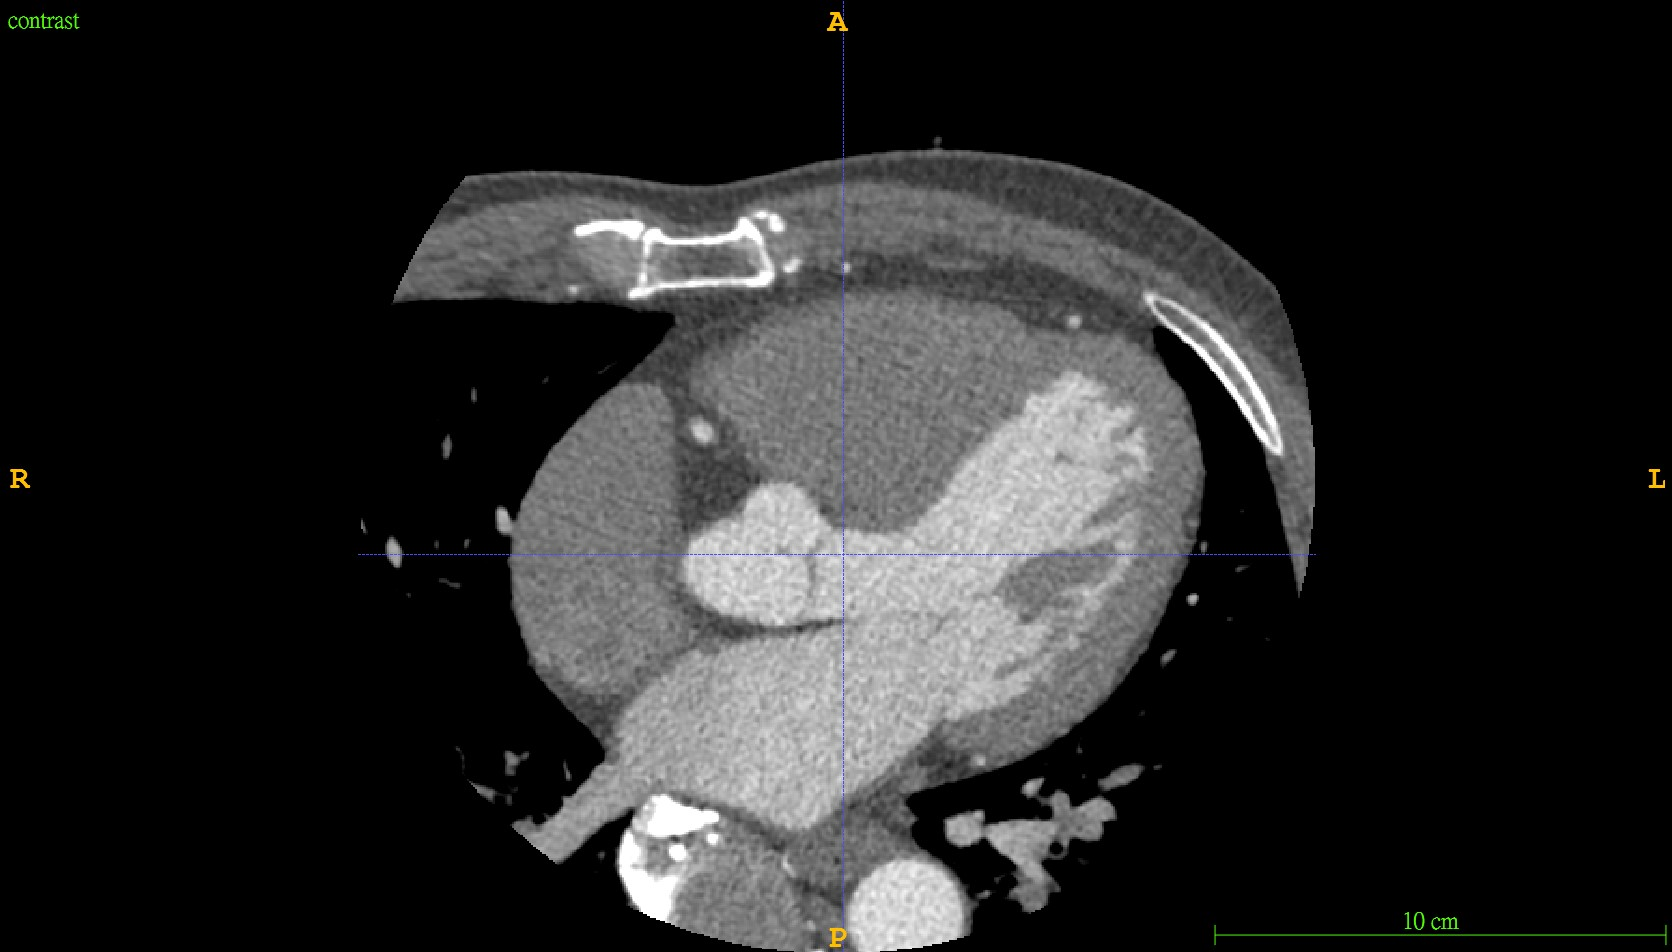
\includegraphics{fig-sample-gan-1-real-contrast}\\[3pt]
    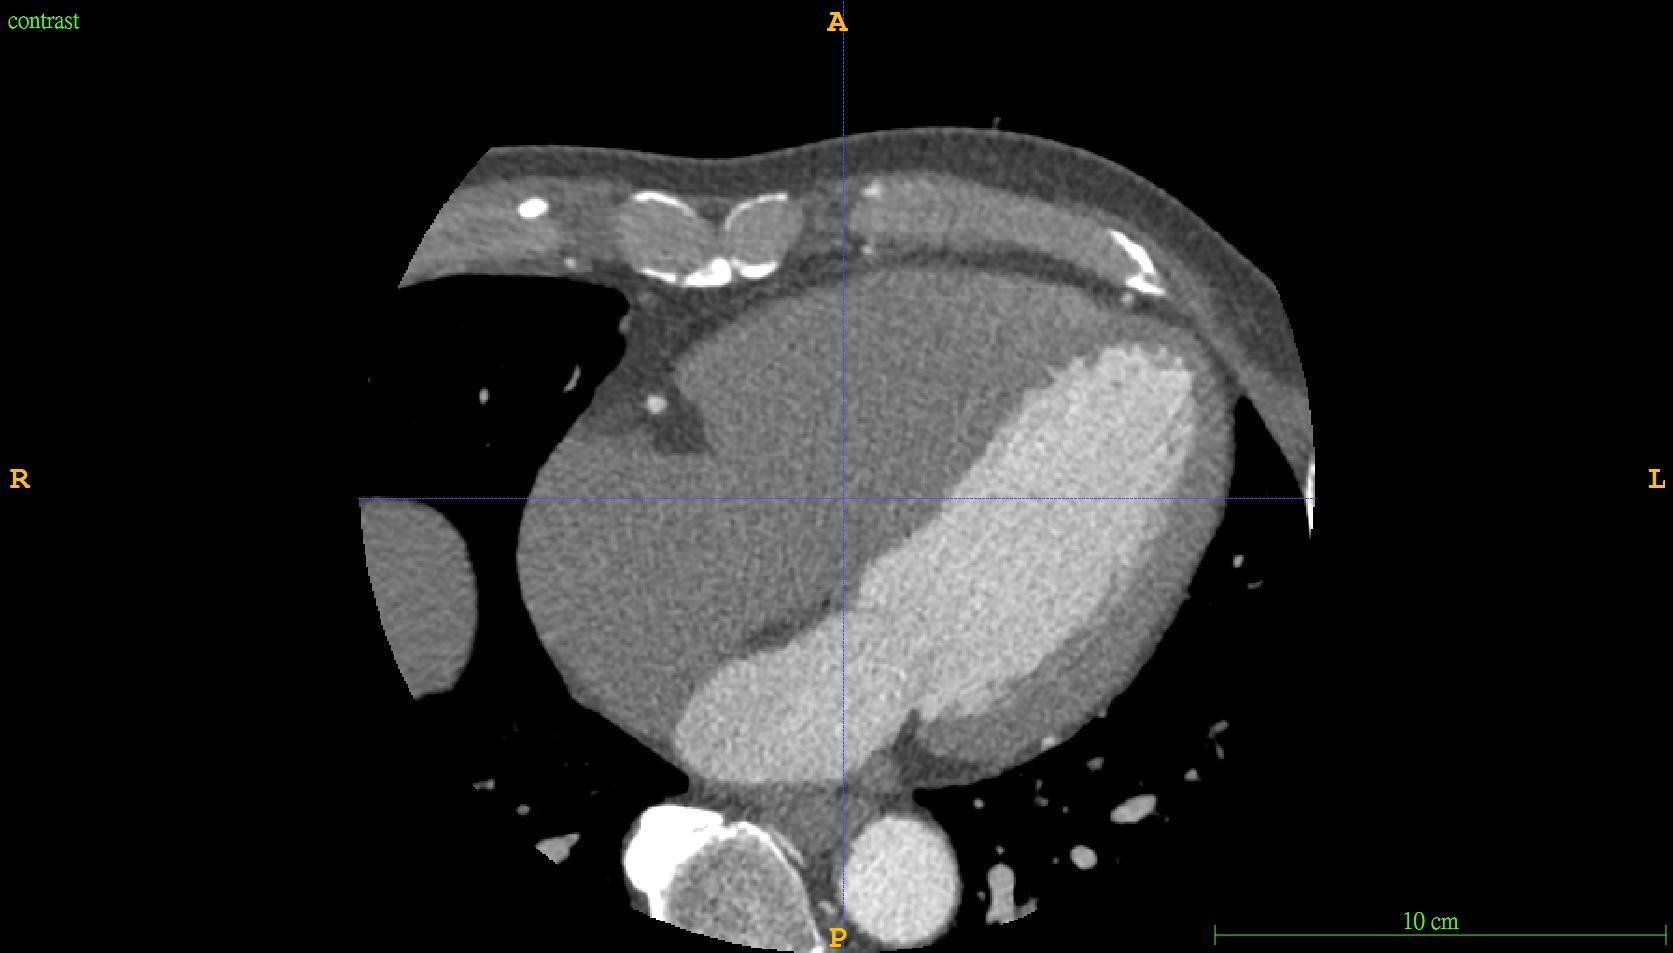
\includegraphics{fig-sample-gan-2-real-contrast}
    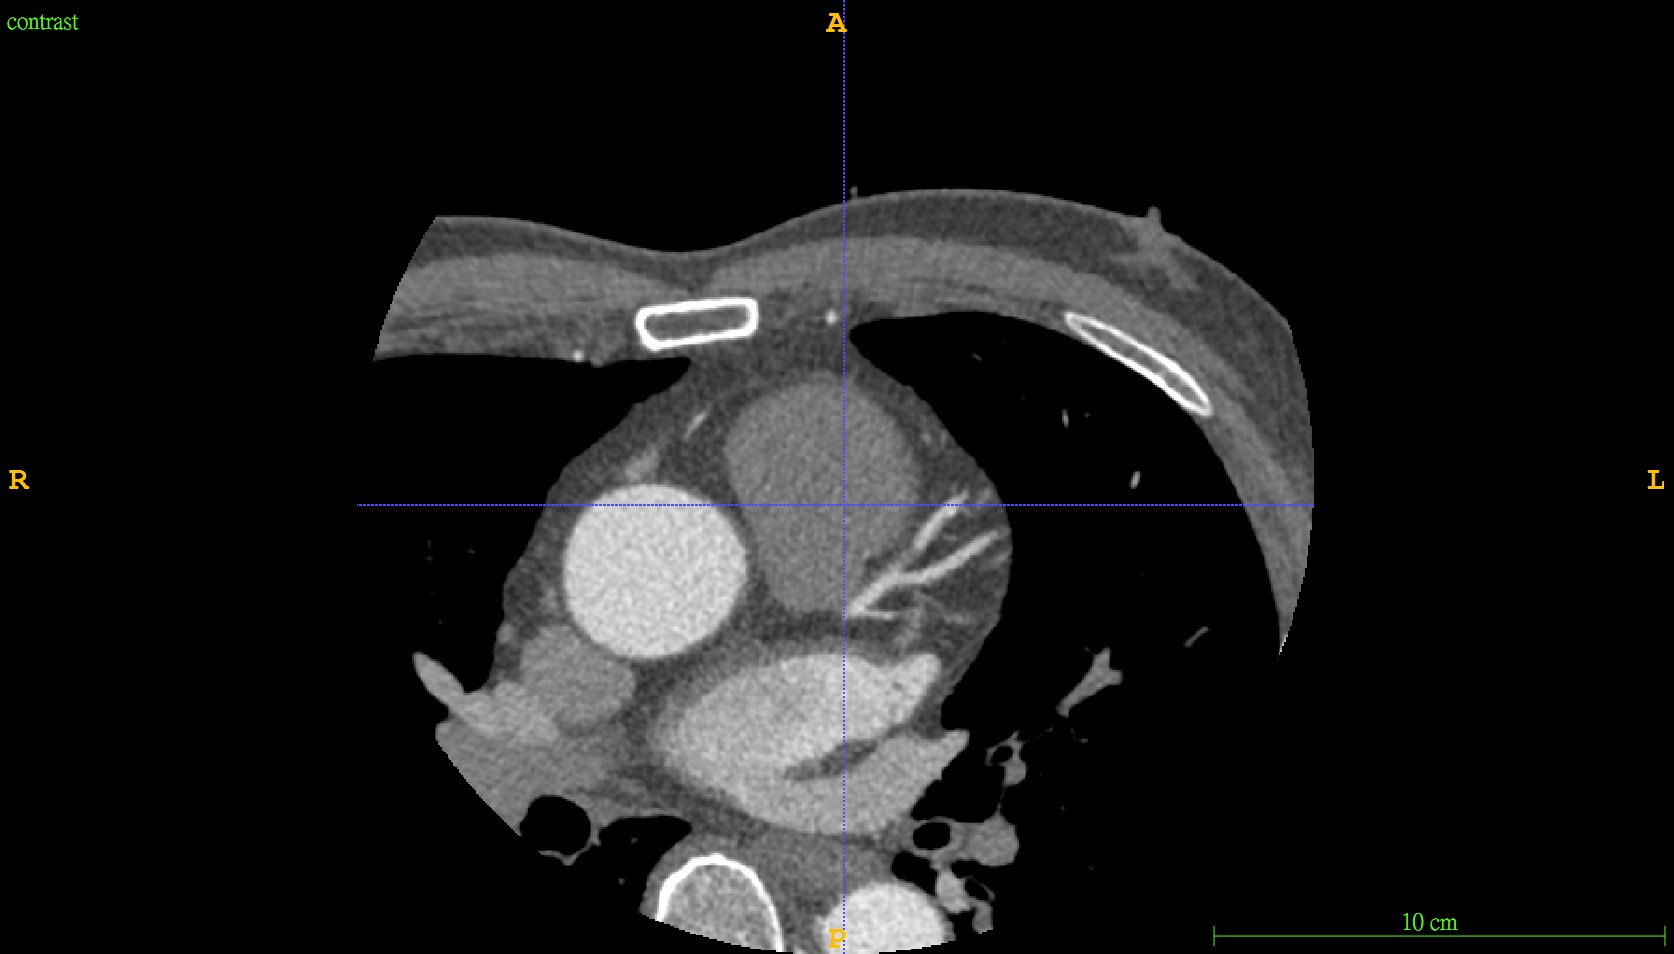
\includegraphics{fig-sample-gan-3-real-contrast}
    \end{subfigure}
    \hfil
    \begin{subfigure}{0.3\linewidth}
        \caption*{CycleGAN產生之無顯影劑增強影像}
    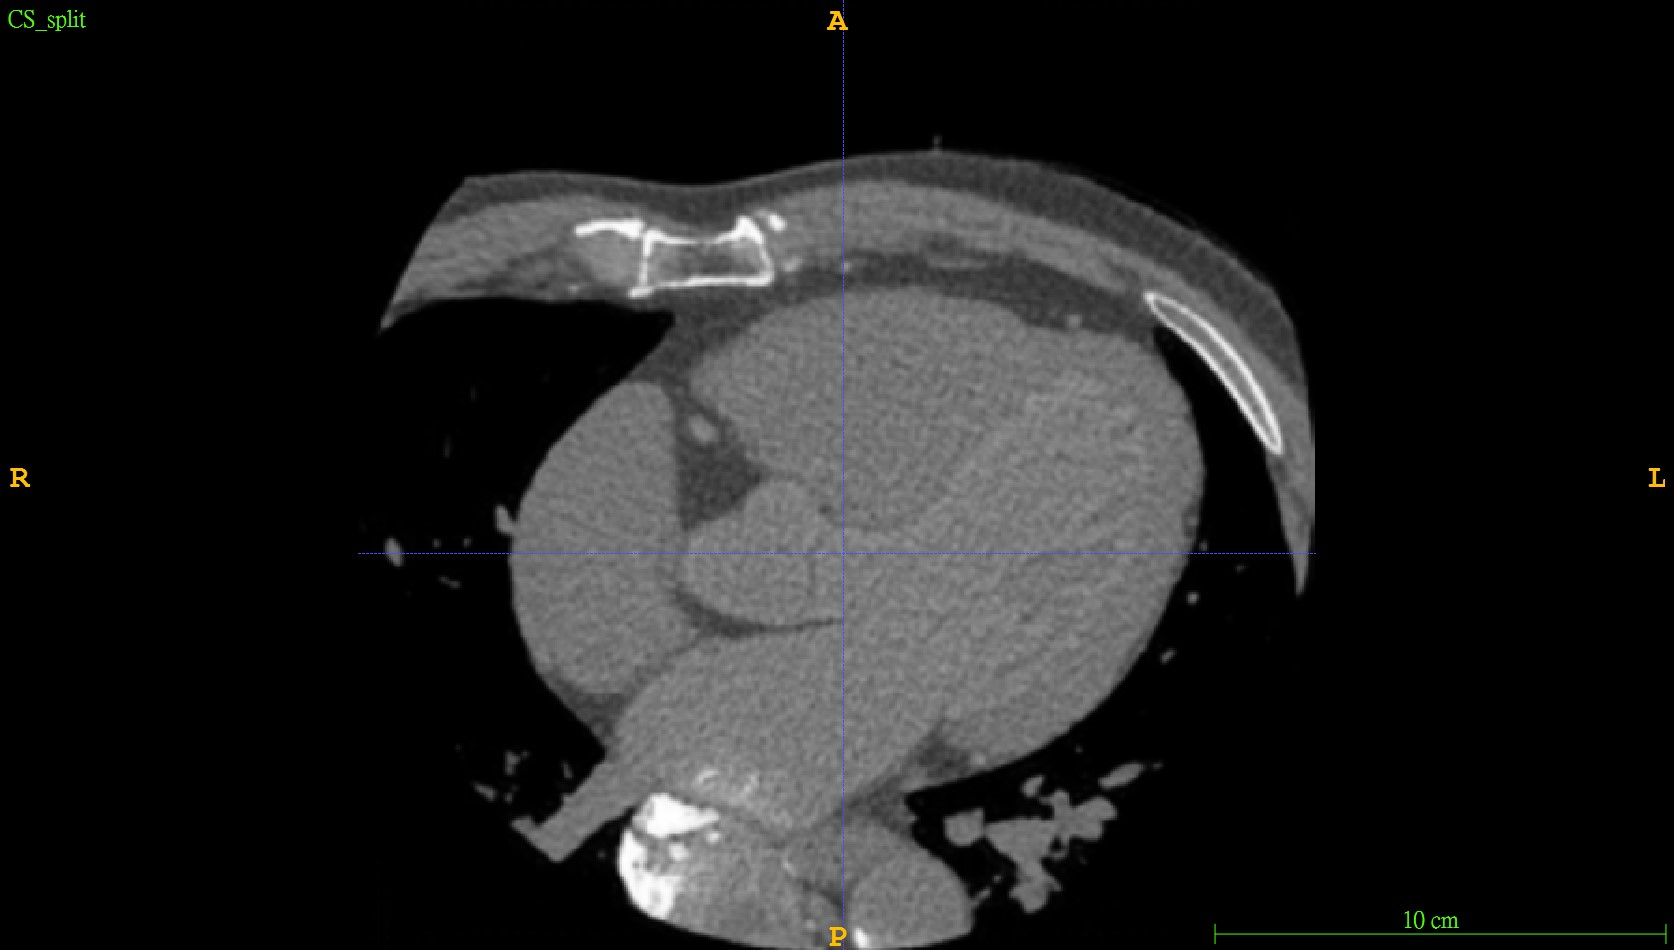
\includegraphics{fig-sample-gan-1-fake-cs}\\[3pt]
    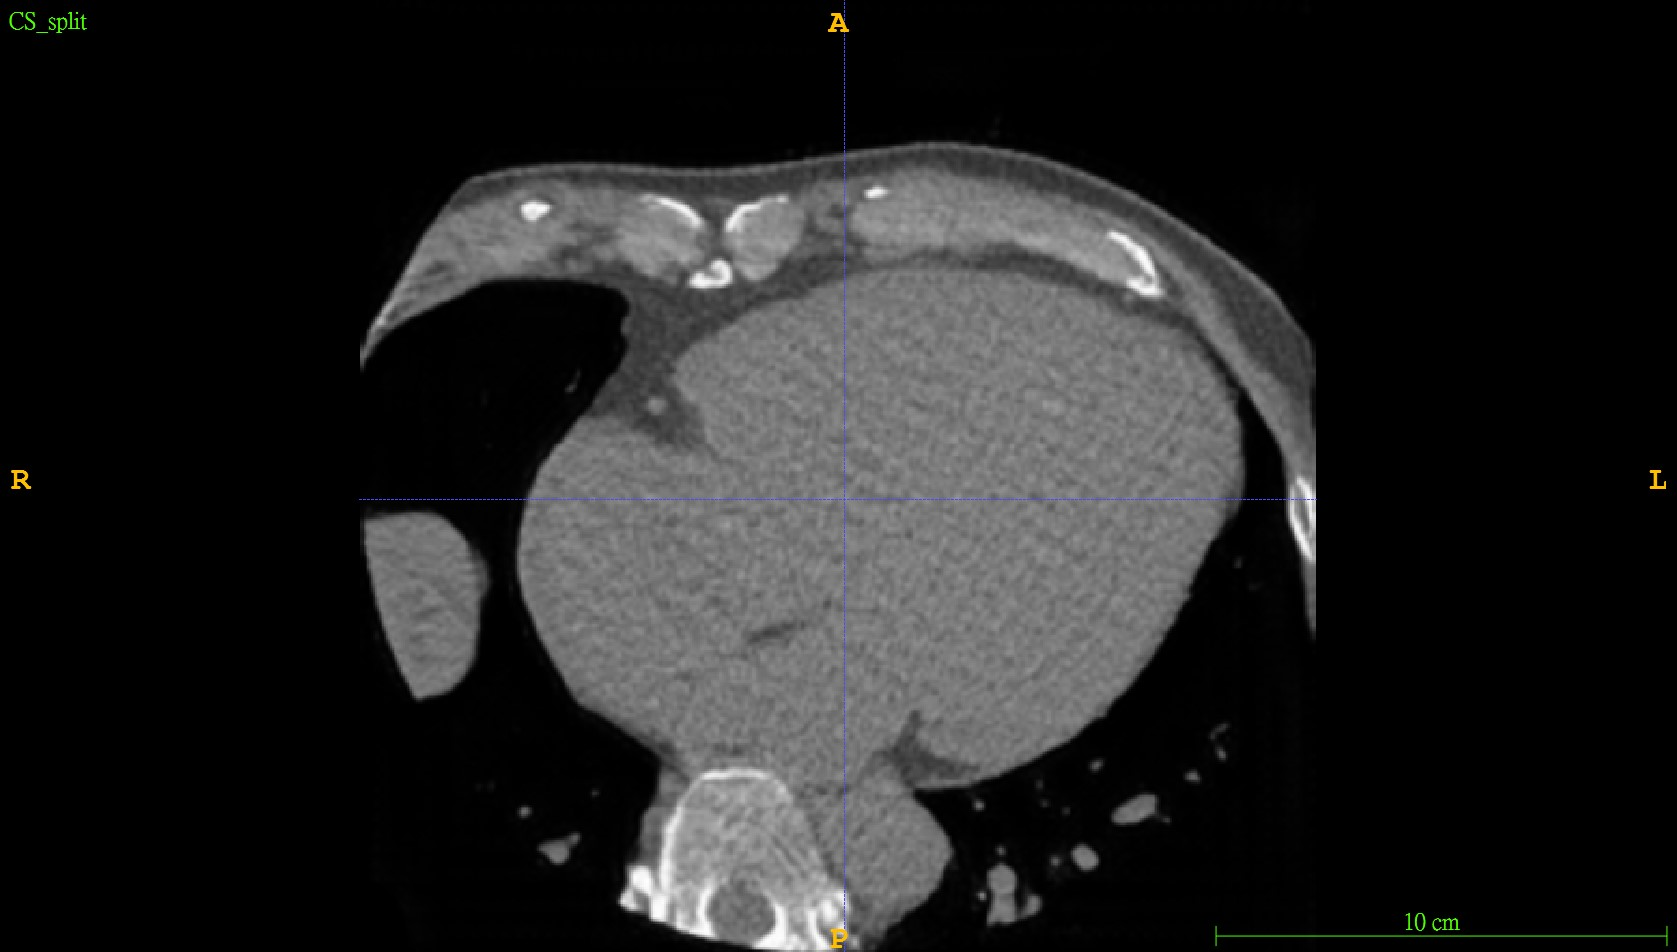
\includegraphics{fig-sample-gan-2-fake-cs}
    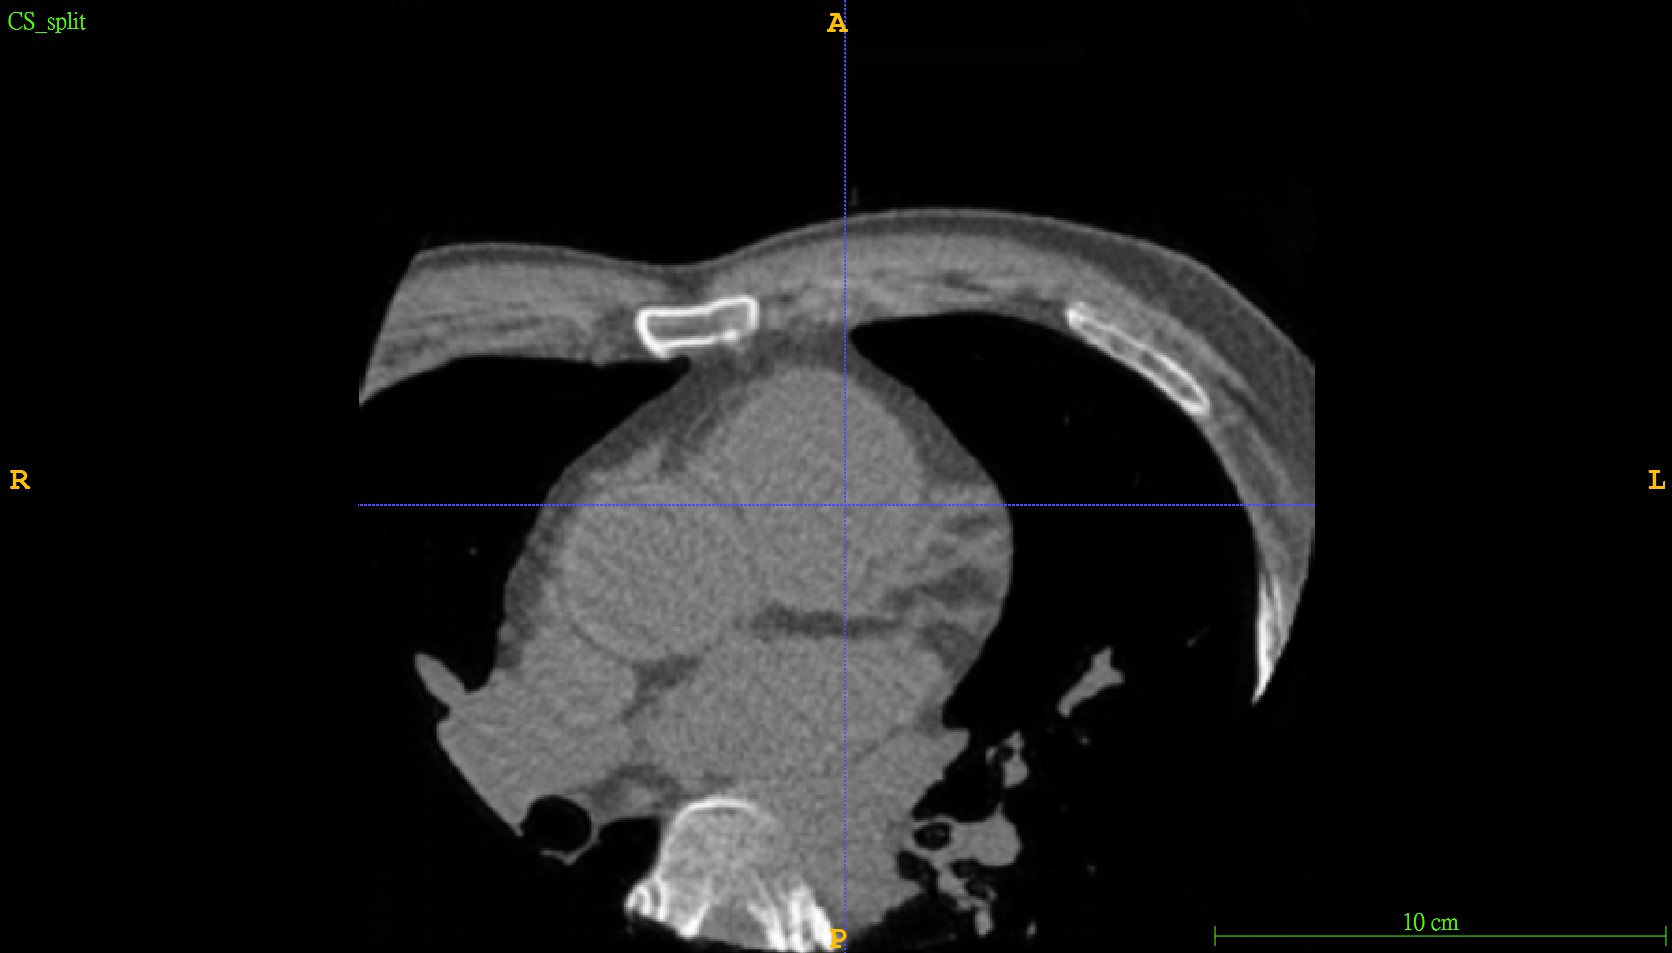
\includegraphics{fig-sample-gan-3-fake-cs}
    \end{subfigure}
    \hfil
    \begin{subfigure}{0.3\linewidth}
        \caption*{真實無顯影劑增強影像}
    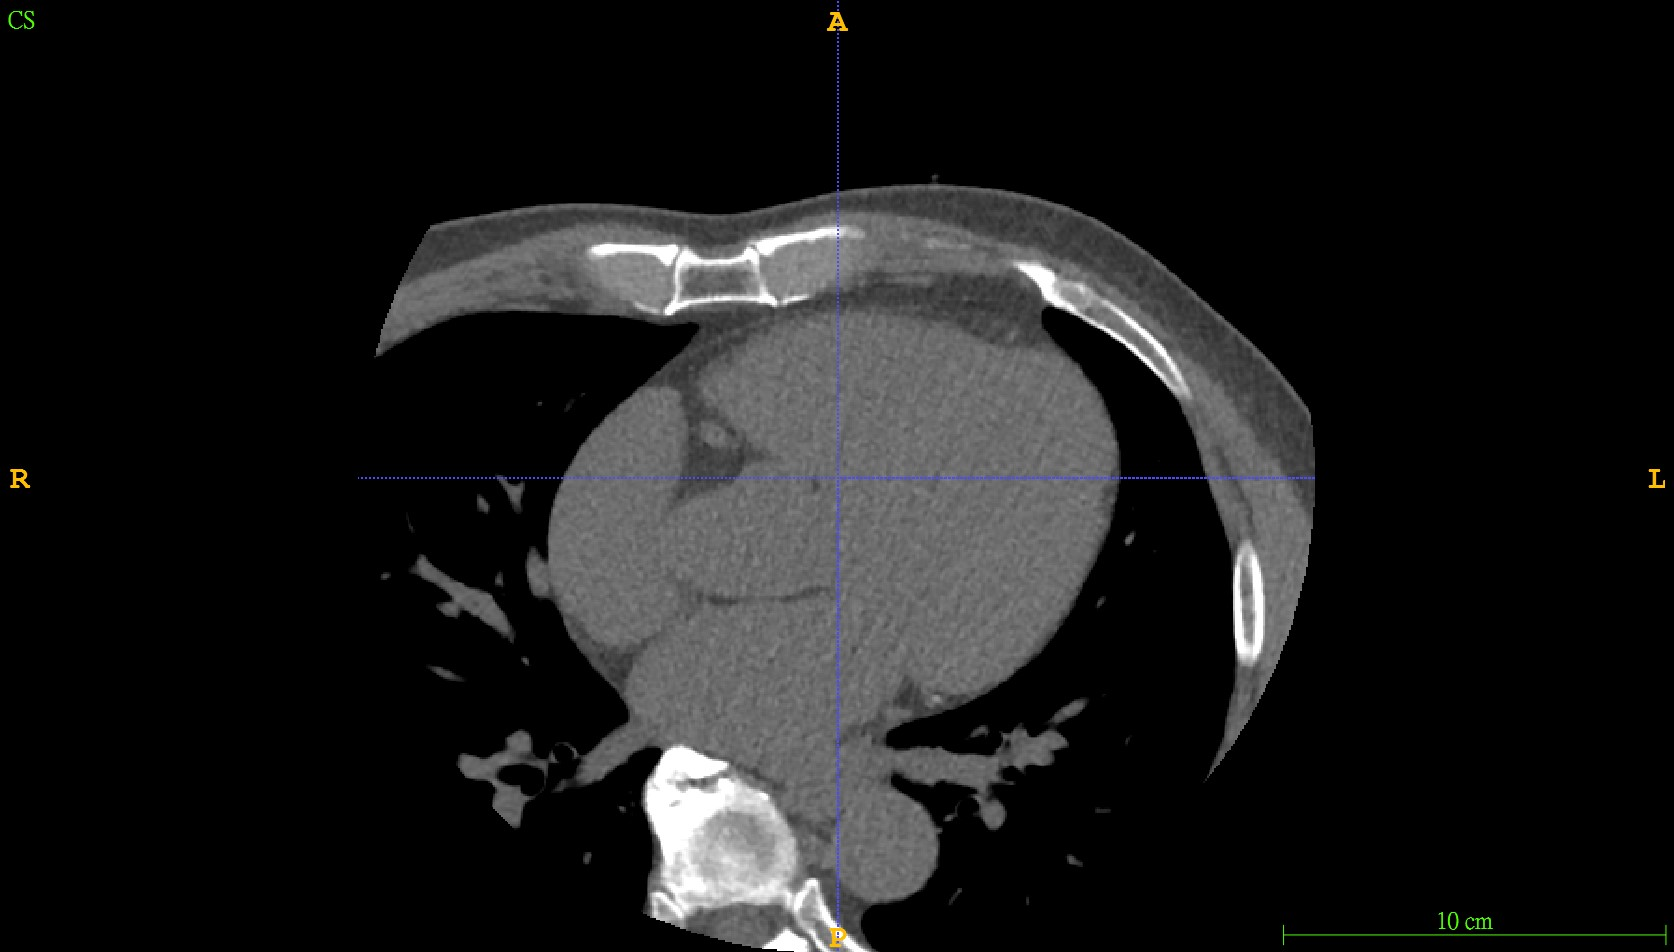
\includegraphics{fig-sample-gan-1-real-cs}\\[3pt]
    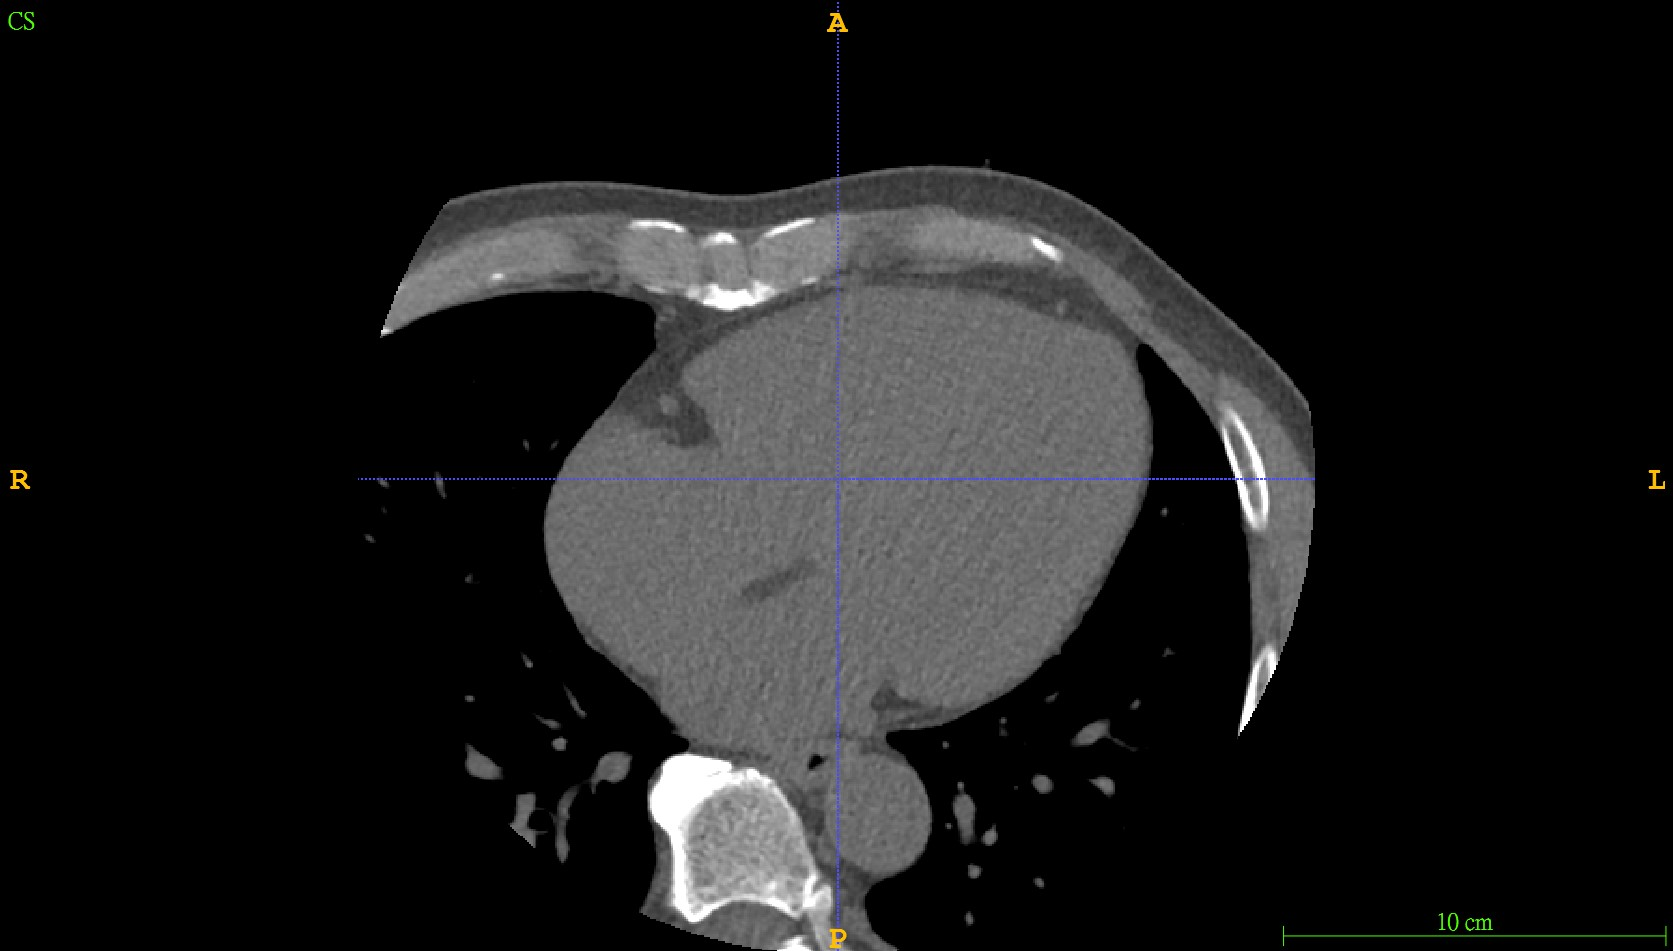
\includegraphics{fig-sample-gan-2-real-cs}
    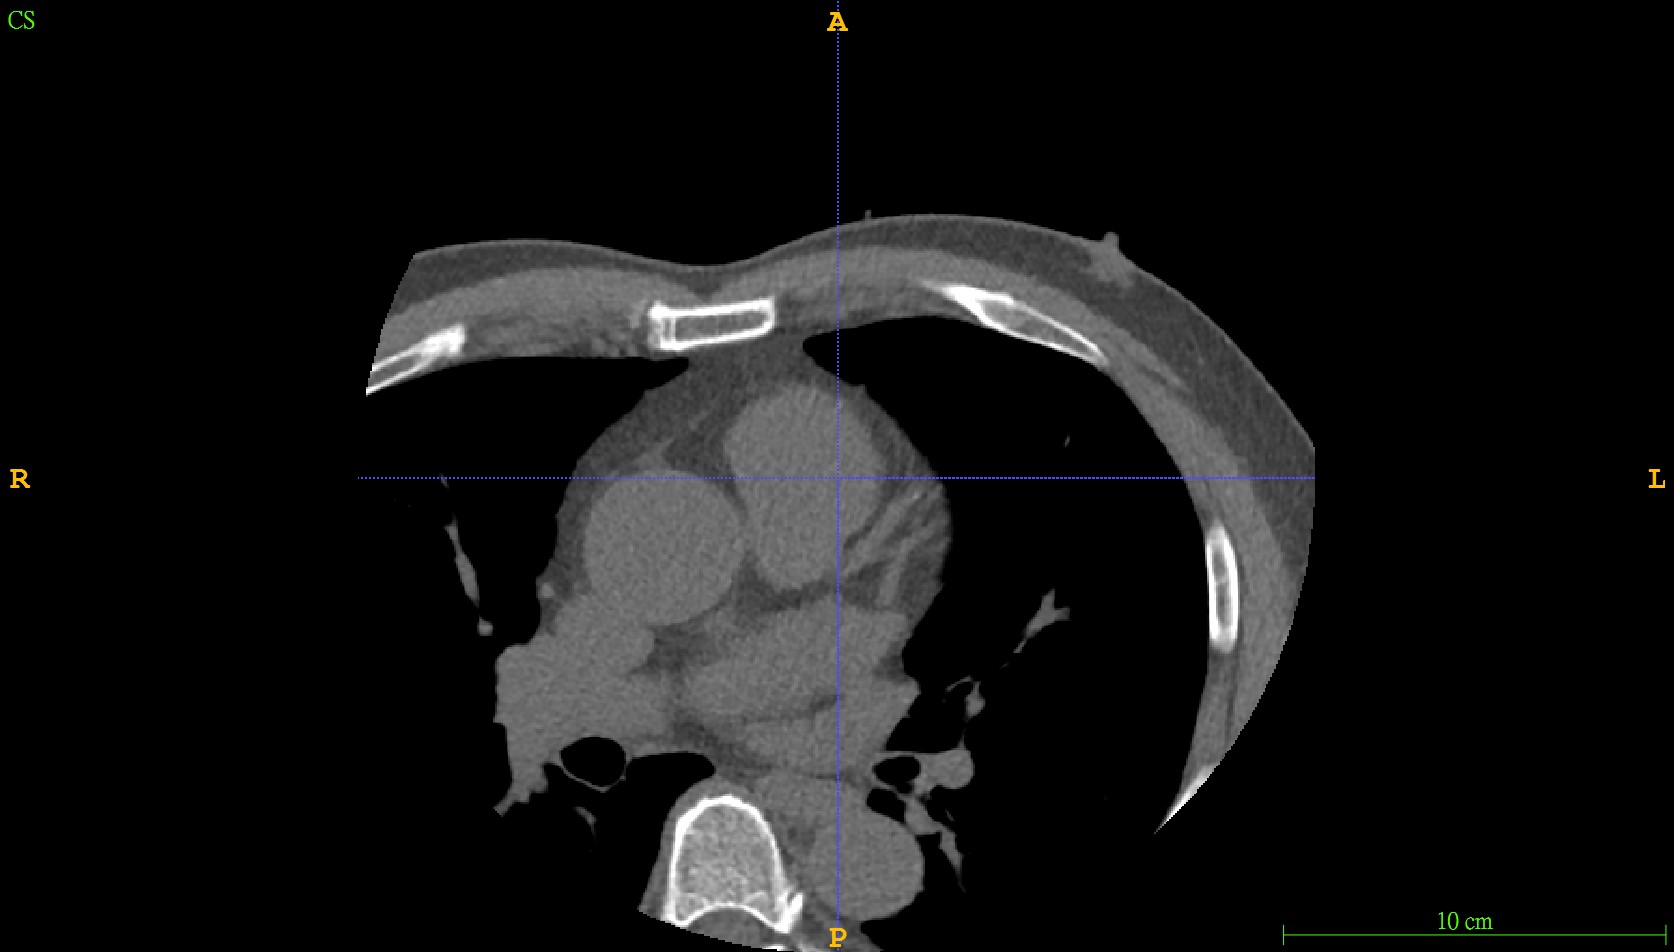
\includegraphics{fig-sample-gan-3-real-cs}
    \end{subfigure}
        \caption{原始影像與CycleGAN轉換結果範例}
    \label{fig:fig-sample-gan}
\end{figure}

於\cref{fig:fig-sample-gan}可以看到CycleGAN能夠確實地將有顯影劑增強之電腦斷層影像中亮度較高之含有顯影劑的血液流經處進行調整,
產生如真實無顯影劑增強電腦斷層影像的結果,
這邊需要注意的是,雖然\cref{fig:fig-sample-gan}中,
每一列有顯影劑增強與無顯影劑增強之電腦斷層影像來自於同一個案,
但由於是不同時間進行的電腦斷層掃描攝影,
因此影像中兩者心臟組織結構無法完全重合。

本研究利用訓練完成之CycleGAN模型將已標記之有顯影劑增強電腦斷層影像進行轉換,
產生虛擬的無顯影劑增強電腦斷層影像資料,
並在無顯影劑增強電腦斷層影像冠狀動脈分割實驗中做為擴增資料集,
以評估資料擴增方法是否能有效提升模型效果。

\section{無顯影劑增強影像之冠狀動脈分割}

本研究利用10組已標註冠狀動脈的無顯影劑增強之電腦斷層影像,
訓練已有顯影劑增強之電腦斷層影像進行冠狀動脈分割之3D U-Net模型,
由於實驗樣本數較少,本研究以K-fold交叉驗證方式進行實驗,
其中8組做為訓練資料,2組做為測試資料,
總共分為5個Fold進行實驗。
\cref{fig:fig-dataset-cs-input-example}為訓練資料範例,
此外,本實驗利用CycleGAN將7組有顯影劑增強之電腦斷層影像轉換為虛擬的無顯影劑增強電腦斷層影像
,做為額外的資料加入訓練,並比較有無使用CycleGAN進行資料擴增對於模型效果的影響。
%,其中\cref{fig:fig-dataset-cs-512-label}為冠狀動脈標記以之三維影像呈現的結果。
\begin{figure}[!hbt]
    %\captionsetup[subfigure]{labelformat=empty} % 完全隱藏圖號
    \centering
    \subcaptionbox
        {由下往上方向
        \label{fig:fig-dataset-cs-512-S}}
        {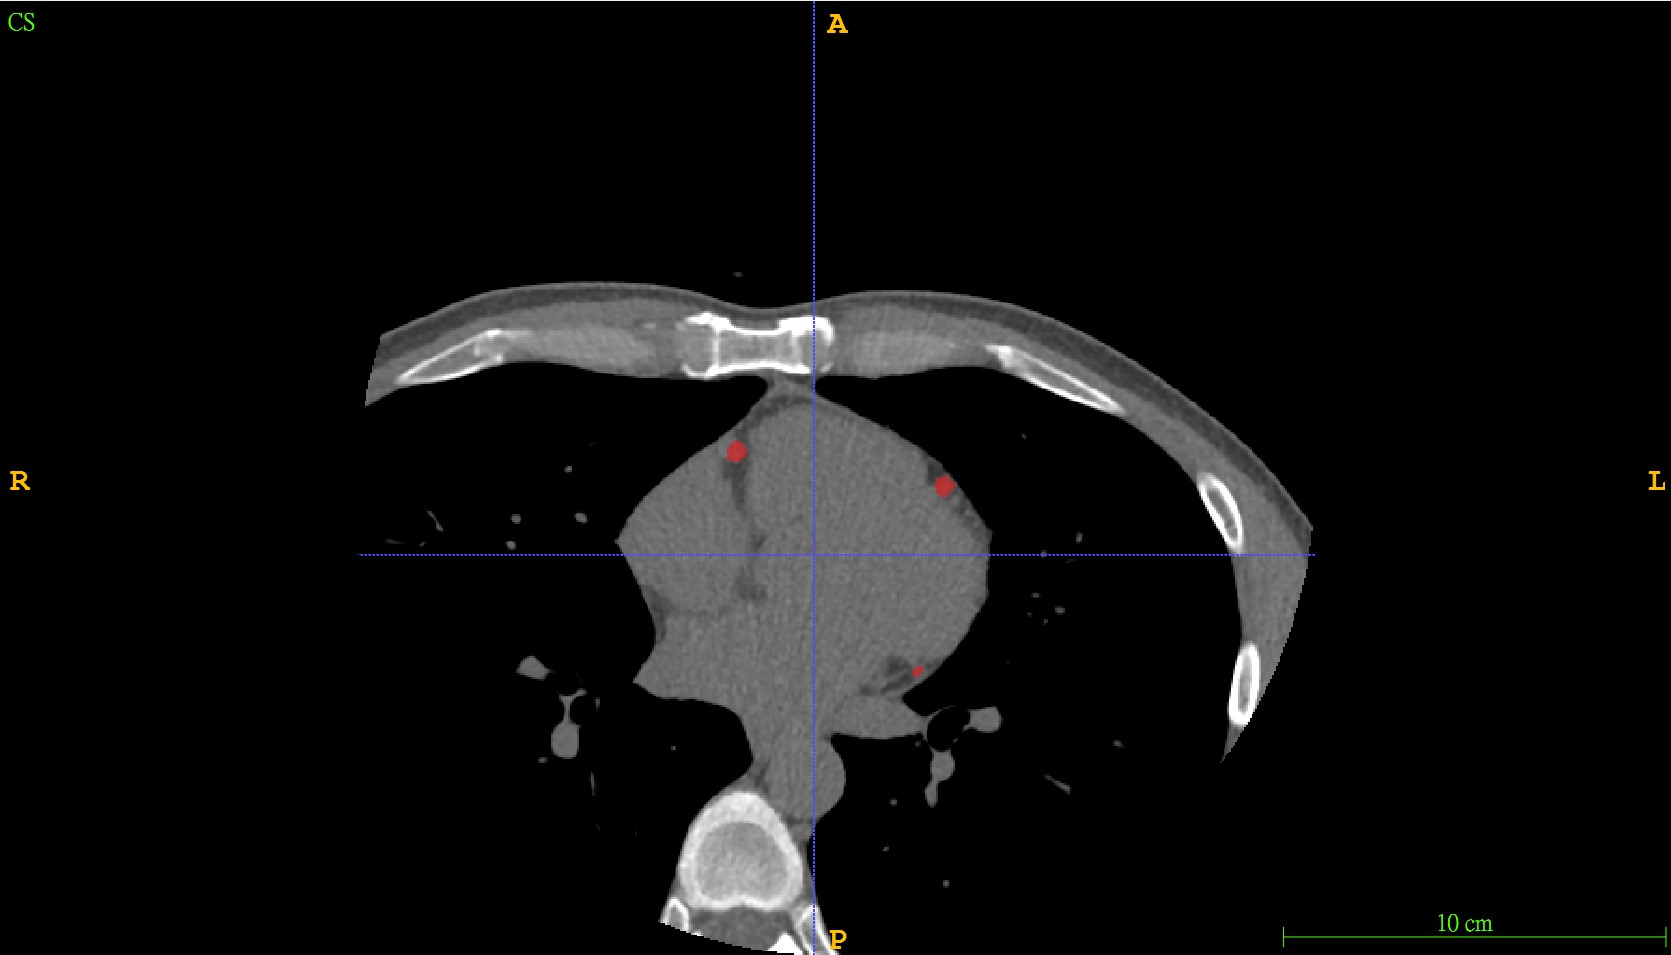
\includegraphics[width=0.475\linewidth]{fig-dataset-cs-512-S.jpg}}
    ~
    \subcaptionbox
        {由左往右方向
        \label{fig:fig-dataset-cs-512-R}}
        {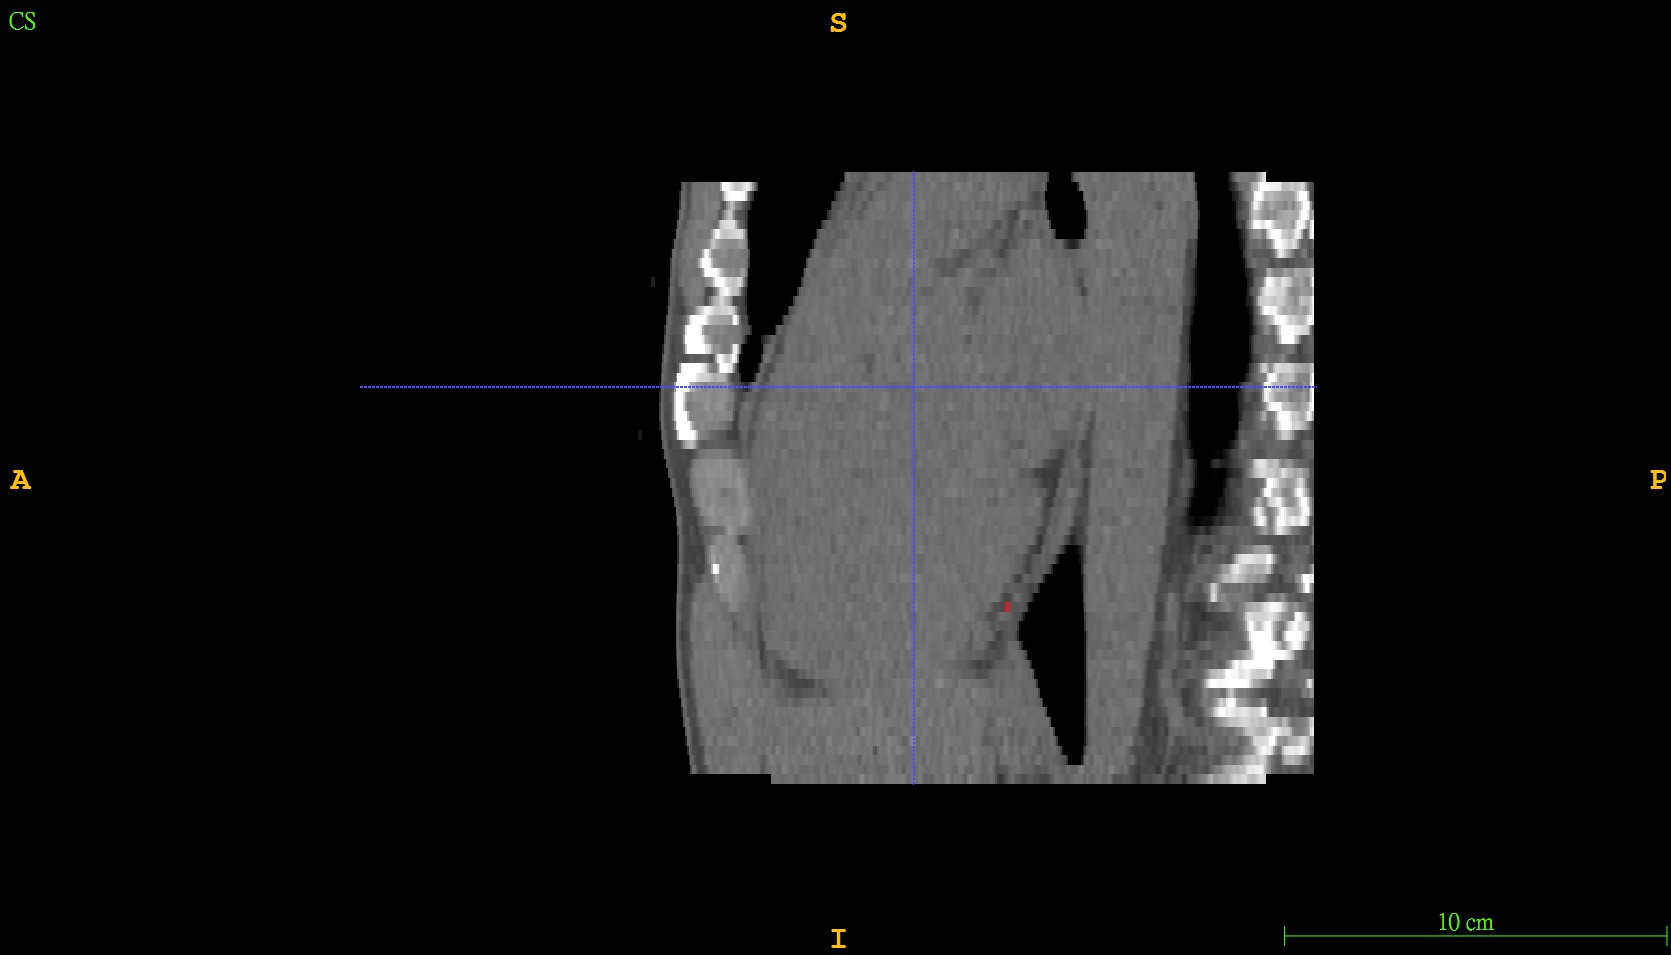
\includegraphics[width=0.475\linewidth]{fig-dataset-cs-512-R.jpg}}
    \vspace{\baselineskip} % 分隔上下列
    \subcaptionbox
        {由前往後方向
        \label{fig:fig-dataset-cs-512-P}}
        {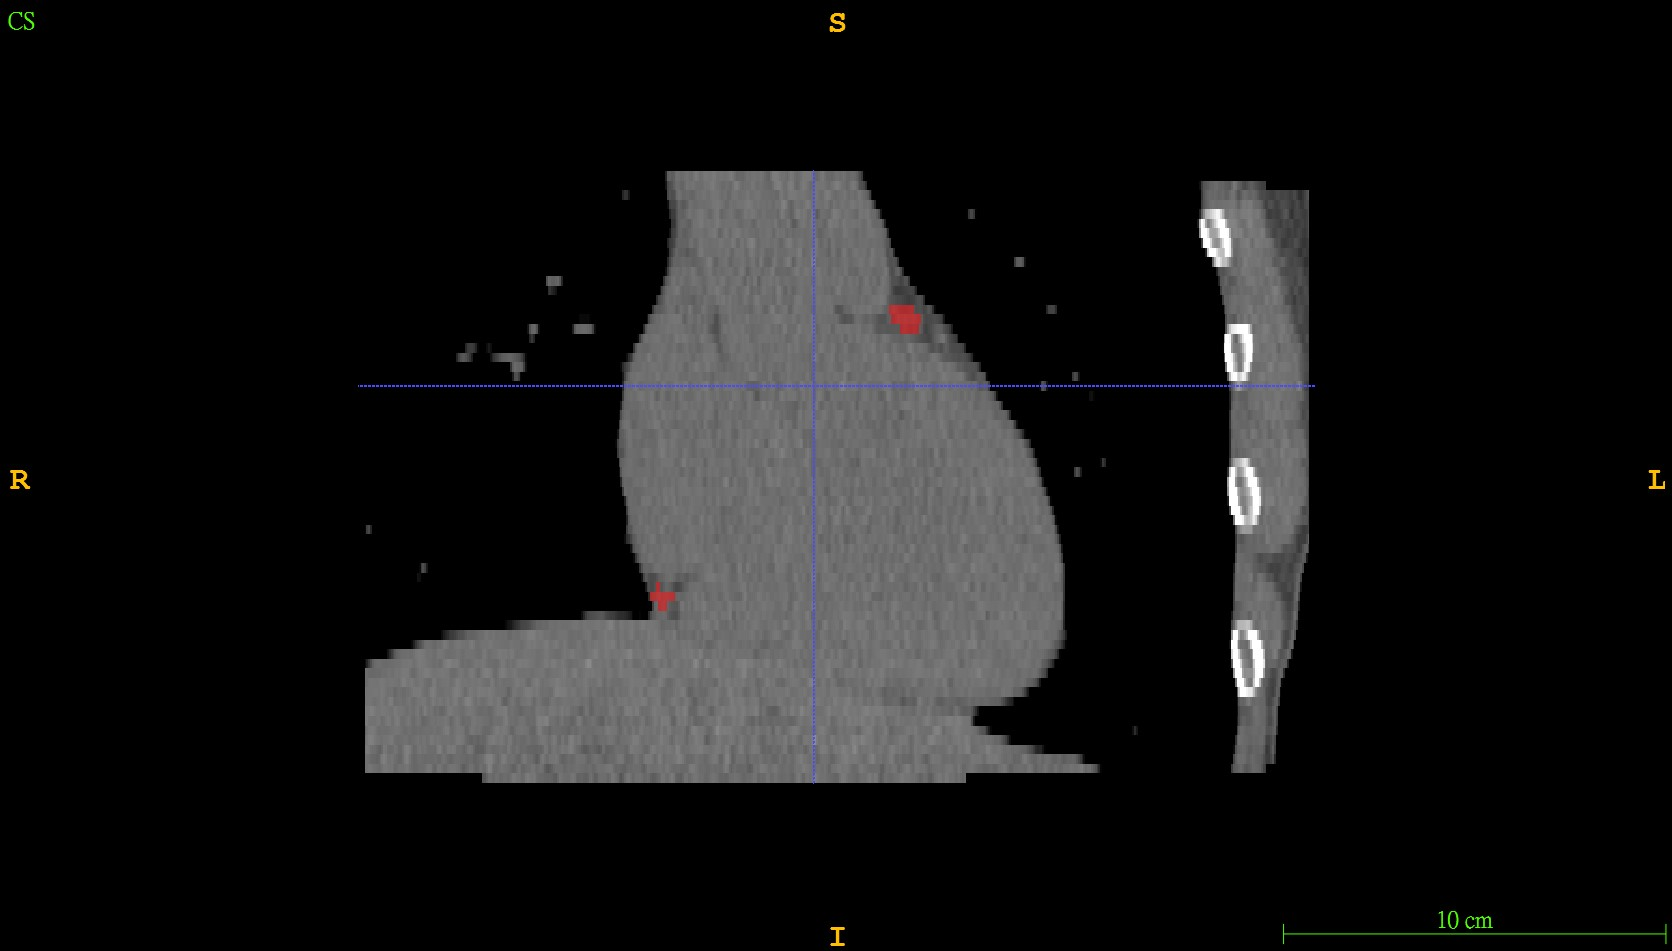
\includegraphics[width=0.475\linewidth]{fig-dataset-cs-512-P.jpg}}
    ~
    \subcaptionbox
        {以三維影像呈現之冠狀動脈標註
        \label{fig:fig-dataset-cs-512-label}}
        {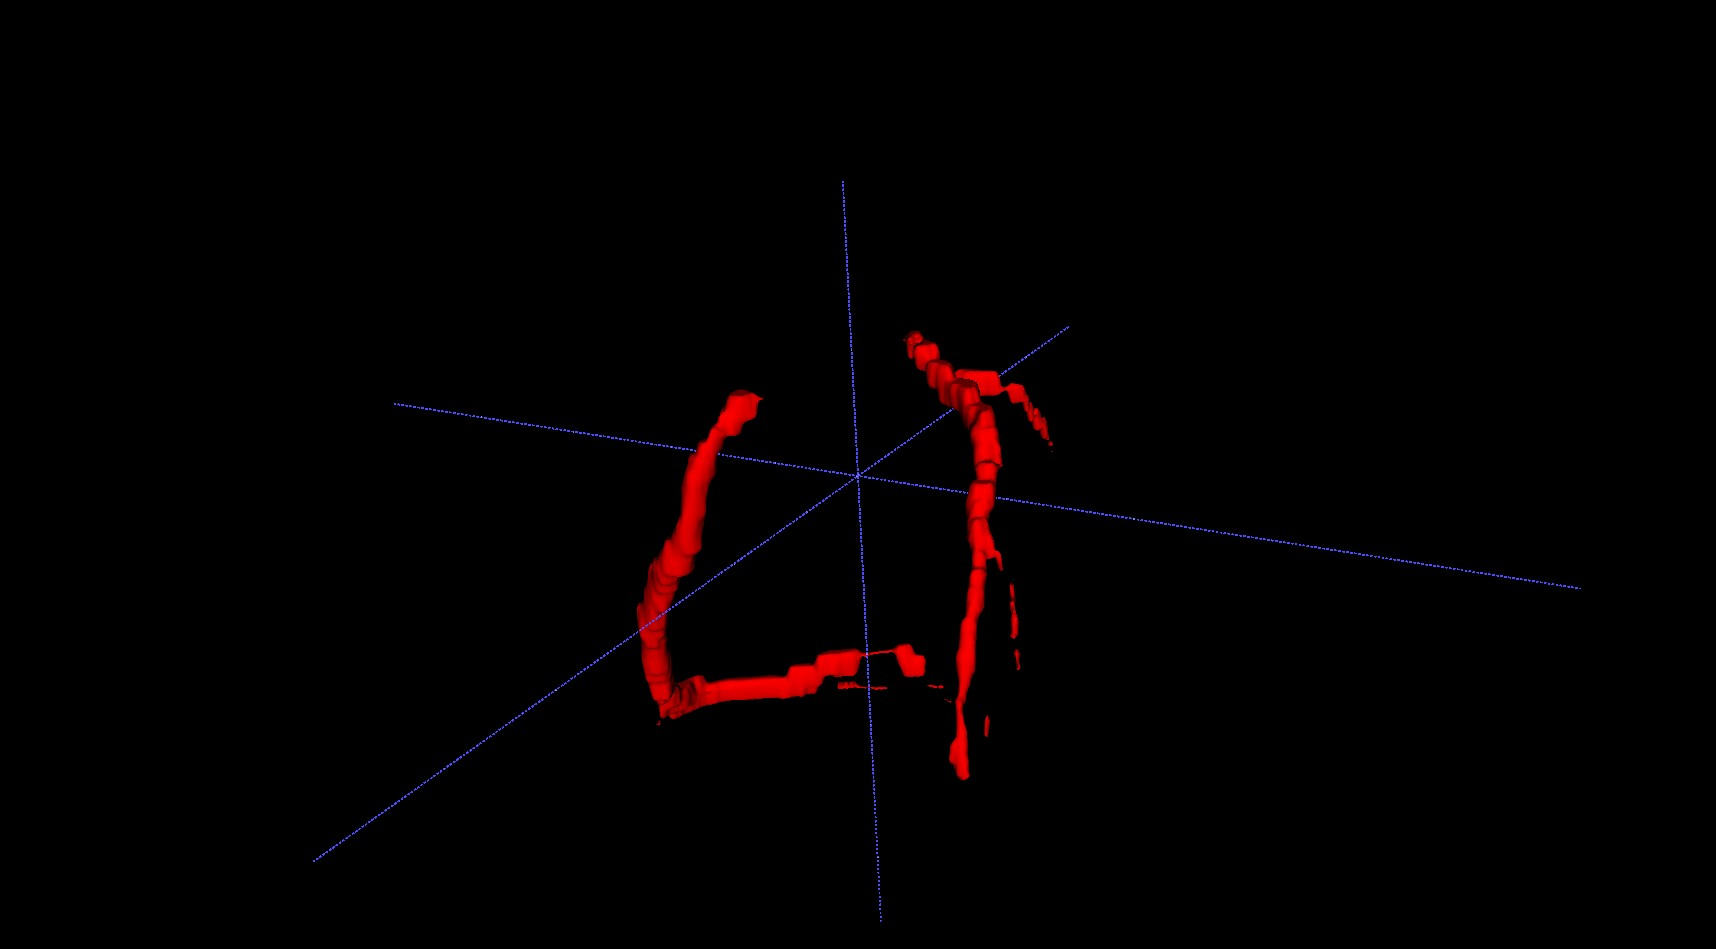
\includegraphics[width=0.475\linewidth]{fig-dataset-cs-512-label.jpg}}
    \caption{模型訓練資料範例-無顯影劑增強}
    \label{fig:fig-dataset-cs-input-example}
\end{figure}

\cref{table:table-cs-only-result}為僅使用無顯影劑之原始資料進行訓練之模型結果,
對於測試資料集平均可以達到Dice Coefficient 0.5158的結果,
\cref{table:table-cs-cyclegan-result}為透過CycleGAN將有顯影劑增強之電腦斷層影像資料轉換為虛擬無顯影劑影像,並且做為擴充訓練資料加入訓練之結果,
如\cref{table:table-cs-cyclegan-result}所示,對於測試資料集平均可以提升至Dice Coefficient 0.5674,
\cref{fig:fig-sample-cs-result-diff-cyclegan}為一僅使用原始資料訓練之模型以及加上CycleGAN資料擴增之模型的結果範例,
可以看到\cref{fig:fig-sample-cs-result-diff-cyclegan-prediction}中使用CycleGAN進行資料擴增之模型能夠分割出更多冠狀動脈結果,
顯示本研究之CycleGAN資料擴增方法能夠有效的輔助模型訓練並提升分割效果。

\begin{table}[h]
    \centering
    \caption{無顯影劑增強之電腦斷層掃描分割結果-僅使用原始資料}
    \label{table:table-cs-only-result}
    \begin{tabular}{cc}
    \hline
    Fold & Dice Coefficient \\
    \hline
    1 & 0.5396 \\
    2 & 0.5164 \\
    3 & 0.5017 \\
    4 & 0.5373 \\
    5 & 0.4842 \\
    \hline
    Average & 0.5158 \\
    \hline
    \end{tabular}
\end{table}

\begin{table}[h]
    \centering
    \caption{無顯影劑增強之電腦斷層掃描分割結果-使用CycleGAN進行資料擴增}
    \label{table:table-cs-cyclegan-result}
    \begin{tabular}{cc}
    \hline
    Fold & Dice Coefficient \\
    \hline
    1 & 0.6155 \\
    2 & 0.5345 \\
    3 & 0.5330 \\
    4 & 0.6251 \\
    5 & 0.5287 \\
    \hline
    Average & \textbf{0.5674} \\
    \hline
    \end{tabular}
\end{table}



\begin{figure}[!hbt]
    %\captionsetup[subfigure]{labelformat=empty} % 完全隱藏圖號
    \centering
    \subcaptionbox
        {人工標註結果
        \label{fig:fig-sample-cs-result-diff-label}}
        {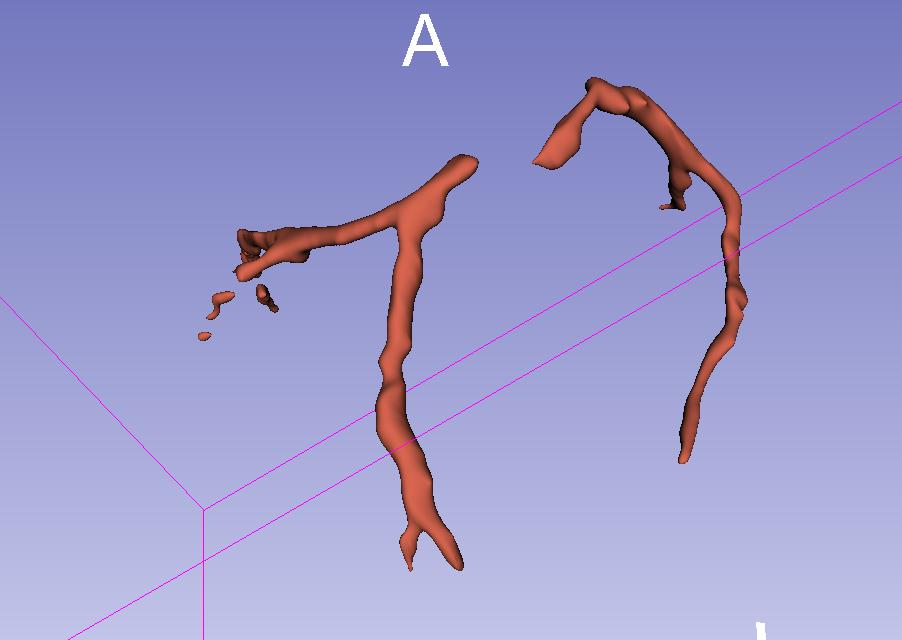
\includegraphics[width=0.3\linewidth]{fig-sample-cs-result-diff-label.jpg}}
    ~
    \subcaptionbox
        {僅使用原始資料之模型輸出結果
        \label{fig:fig-sample-cs-result-diff-only-cs-prediction}}
        {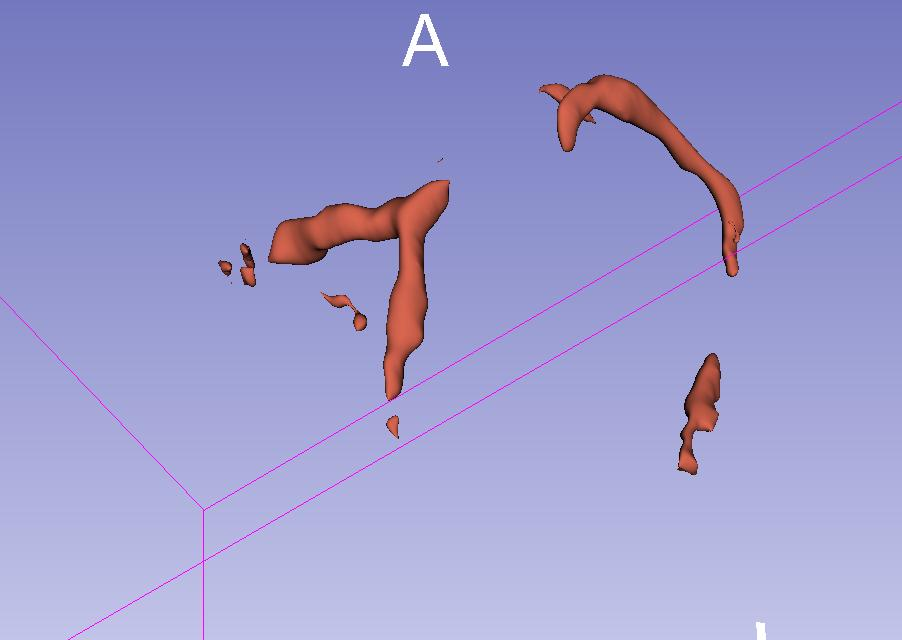
\includegraphics[width=0.3\linewidth]{fig-sample-cs-result-diff-only-cs-prediction.jpg}}
    ~
    \subcaptionbox
        {使用CycleGAN進行資料擴增之模型輸出結果
        \label{fig:fig-sample-cs-result-diff-cyclegan-prediction}}
        {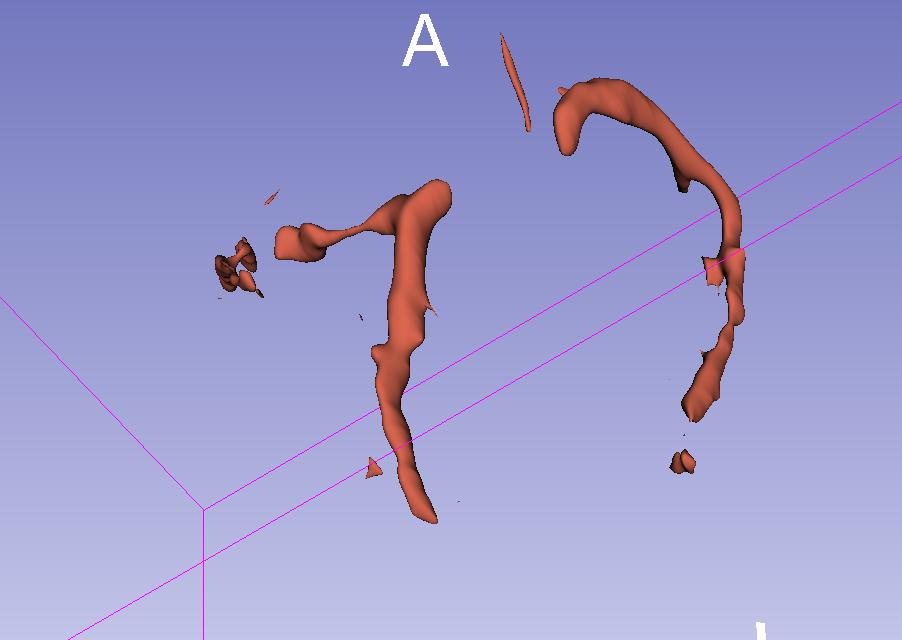
\includegraphics[width=0.3\linewidth]{fig-sample-cs-result-diff-cyclegan-prediction.jpg}}
    \caption{有無使用CycleGAN進行資料擴增之模型輸出結果}
    \label{fig:fig-sample-cs-result-diff-cyclegan}
\end{figure}

雖然CycleGAN資料擴增方法能夠有效的輔助模型訓練並提升分割效果,
但還是與有顯影劑影像的分割結果有所差距,
本研究認為原因包含1. 無顯影劑影像的低對比度性質,
由於沒有顯影劑的幫助,無顯影劑影像中的血管與其他軟組織的對比度較不明顯,
因此其分割難度也較有顯影劑影像高許多,2. 本研究使用的無顯影劑影像為64切,
比起256切的有顯影劑影像之解析度較低,
因此在分割結果上較難達到良好的連續性。

\cref{fig:fig-sample-cs-result-good-1}以及\cref{fig:fig-sample-cs-result-good-2}為模型較佳之輸出結果範例,
可以觀察到在輸出結果中RCA、LAD、LCx的主要結構皆有被分割出來,
模型對於RCA能夠完整地將血管分割出來,
然而LAD與LCx的末端則有較多沒有正確分割出來的結果,
也是模型結果較差的主要原因。


\begin{figure}[!hbt]
    %\captionsetup[subfigure]{labelformat=empty} % 完全隱藏圖號
    \centering
    \subcaptionbox
        {人工標記結果
        \label{fig:fig-sample-cs-result-good-1-label}}
        {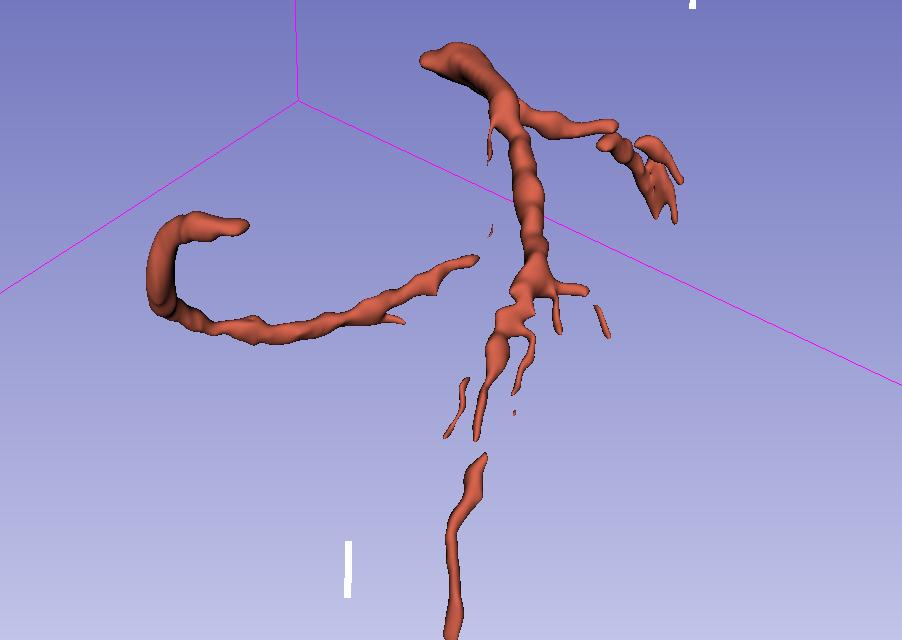
\includegraphics[width=0.475\linewidth]{fig-sample-cs-result-good-1-label.jpg}}
    ~
    \subcaptionbox
        {模型輸出結果
        \label{fig:fig-sample-cs-result-good-1-prediction}}
        {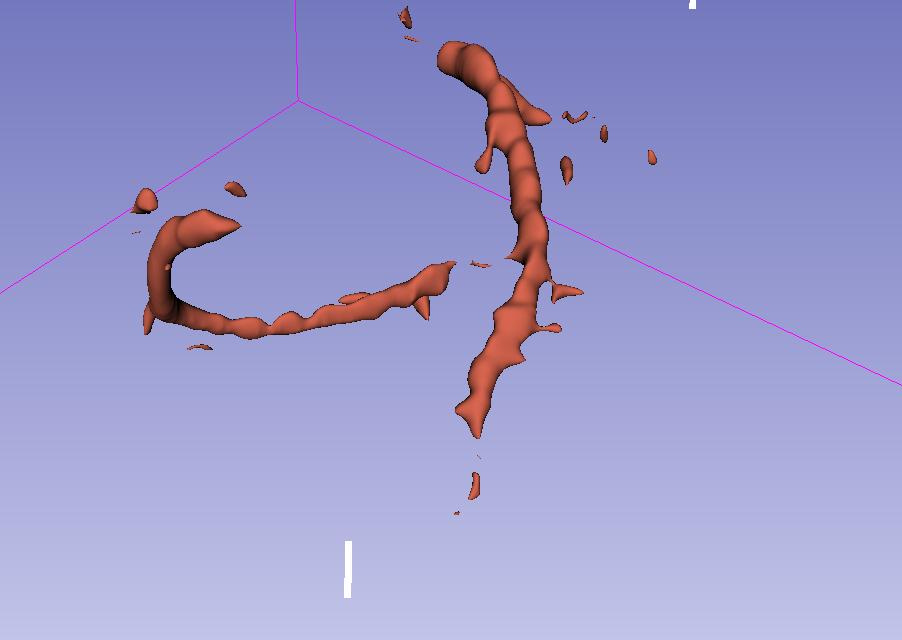
\includegraphics[width=0.475\linewidth]{fig-sample-cs-result-good-1-prediction.jpg}}
    \caption{無顯影劑增強之電腦斷層掃描分割較佳結果-範例1}
    \label{fig:fig-sample-cs-result-good-1}
\end{figure}

\begin{figure}[!hbt]
    %\captionsetup[subfigure]{labelformat=empty} % 完全隱藏圖號
    \centering
    \subcaptionbox
        {人工標記結果
        \label{fig:fig-sample-cs-result-good-1-label}}
        {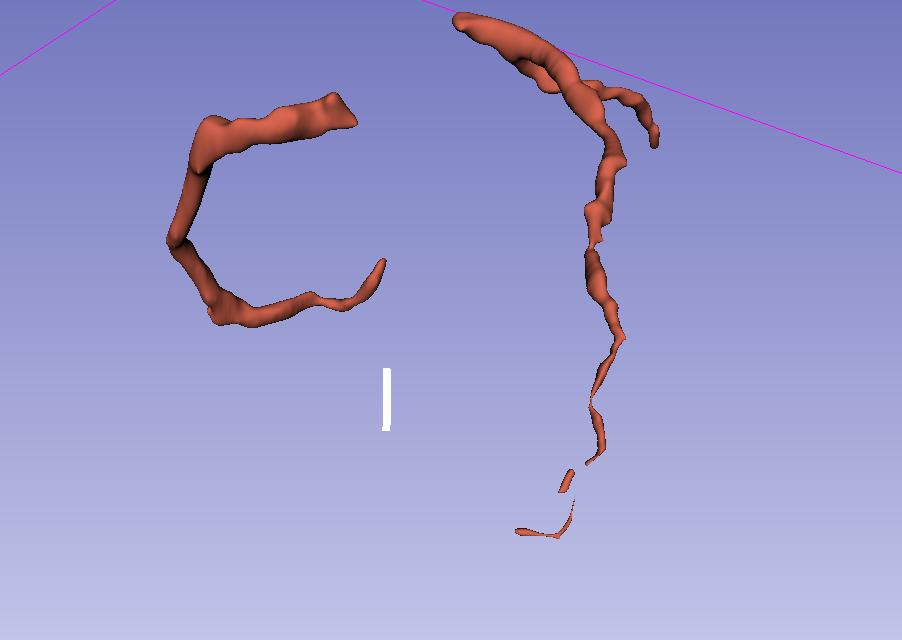
\includegraphics[width=0.475\linewidth]{fig-sample-cs-result-good-2-label.jpg}}
    ~
    \subcaptionbox
        {模型輸出結果
        \label{fig:fig-sample-cs-result-good-1-prediction}}
        {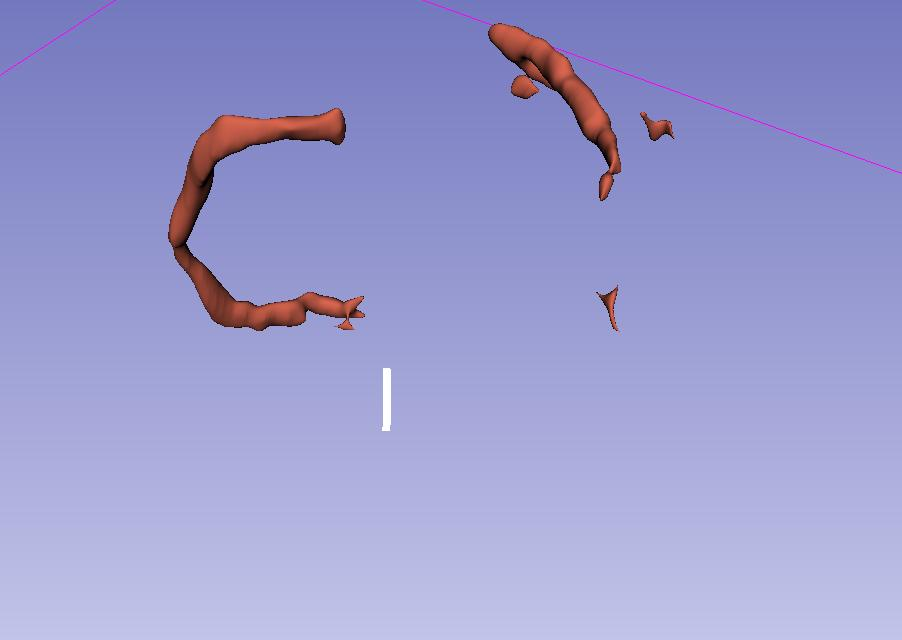
\includegraphics[width=0.475\linewidth]{fig-sample-cs-result-good-2-prediction.jpg}}
    \caption{無顯影劑增強之電腦斷層掃描分割較佳結果-範例2}
    \label{fig:fig-sample-cs-result-good-2}
\end{figure}

\cref{fig:fig-sample-cs-result-bad-1}為一模型較差之輸出結果範例,
可以觀察到在輸出結果中RCA、LAD、LCx的主要結構皆有被分割出來,
然而RCA末端有一段未被分割出來的血管,
且在LAD與LCx有較多的錯誤分割結果,
一些非冠狀動脈的部分也被錯誤地分割出來。

\begin{figure}[!hbt]
    %\captionsetup[subfigure]{labelformat=empty} % 完全隱藏圖號
    \centering
    \subcaptionbox
        {人工標記結果
        \label{fig:fig-sample-cs-result-bad-1-label}}
        {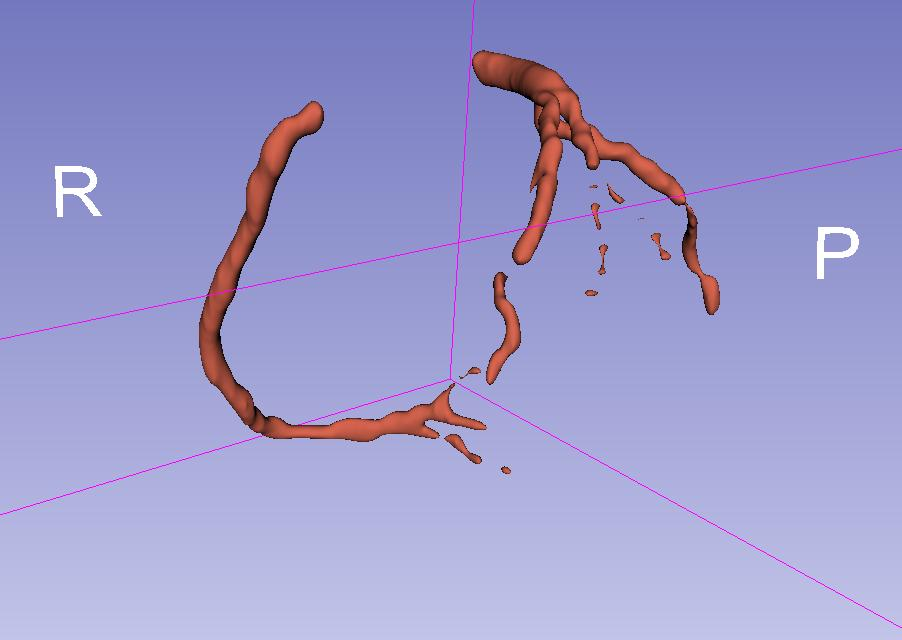
\includegraphics[width=0.475\linewidth]{fig-sample-cs-result-bad-1-label.jpg}}
    ~
    \subcaptionbox
        {模型輸出結果
        \label{fig:fig-sample-cs-result-bad-1-prediction}}
        {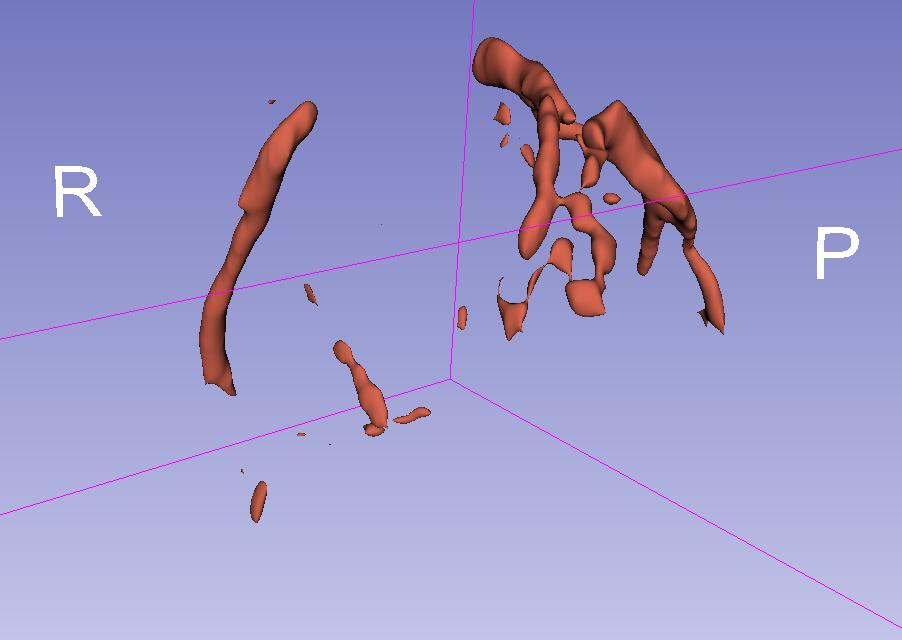
\includegraphics[width=0.475\linewidth]{fig-sample-cs-result-bad-1-prediction.jpg}}
    \caption{無顯影劑增強之電腦斷層掃描分割較差結果範例}
    \label{fig:fig-sample-cs-result-bad-1}
\end{figure}

雖然無顯影劑之冠狀動脈分割結果相較於有顯影劑之結果有一些差距,
不過顯影劑之冠狀動脈分割模型還是能分割出大致的冠狀動脈結構如RCA、LAD、LCx的主要分支,
對於不適合注射顯影劑而只能取得無顯影劑電腦斷層影像的受檢者,
本研究之無顯影劑冠狀動脈分割模型能夠增強無顯影劑影像的利用價值,
做為額外參考資訊提供給醫師,使得在診斷時可以更了解受檢者之冠狀動脈結構。

% 
% 
% \begin{figure}[!ht]
%     \centering
%     \setkeys{Gin}{width=\linewidth}
%     \begin{subfigure}{0.45\textwidth}
%         \caption*{人工標註結果}
%     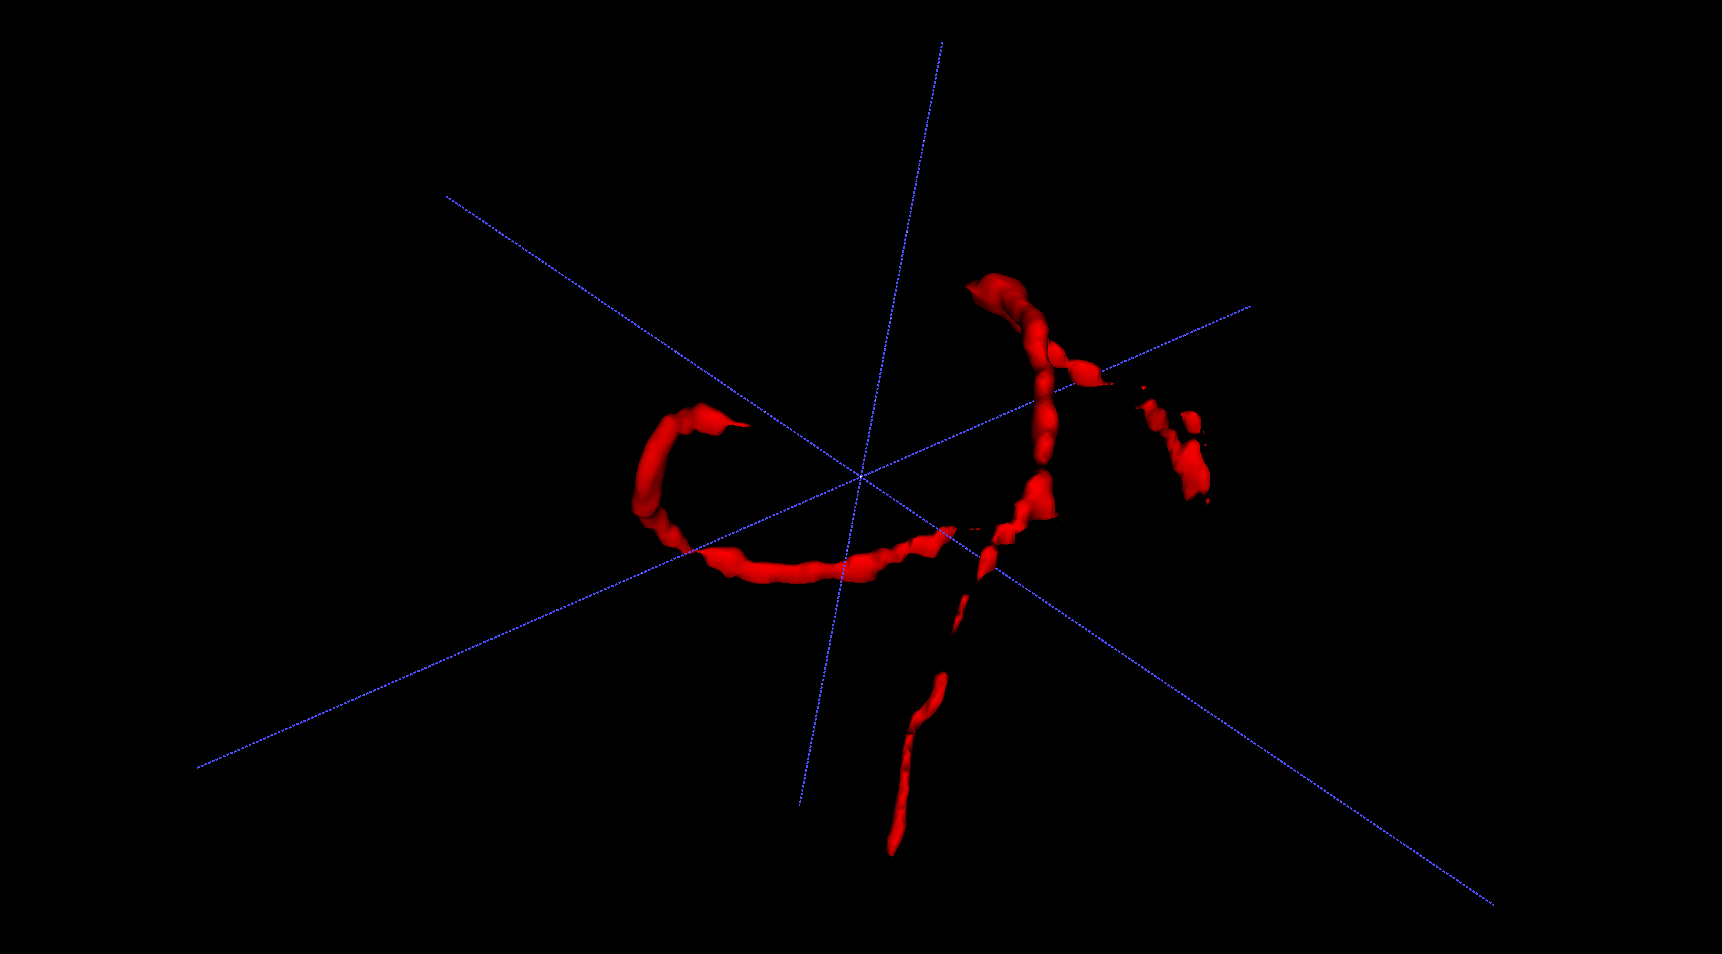
\includegraphics{fig-sample-cs-result-1-label}\\[3pt]
%     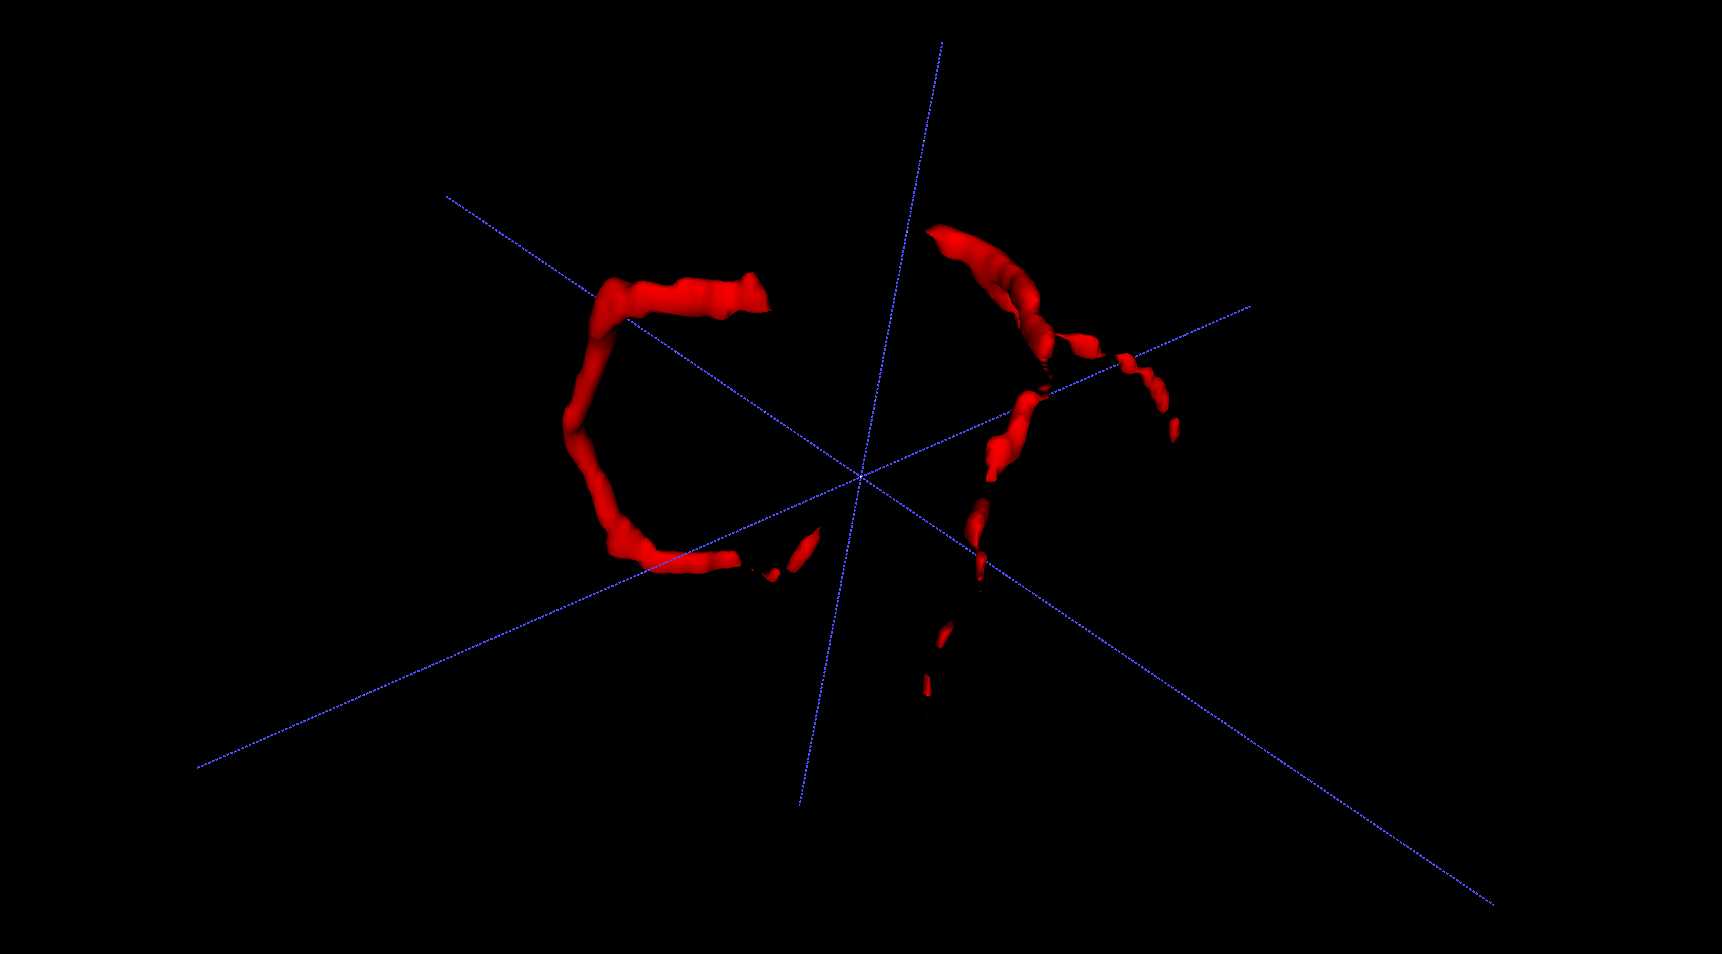
\includegraphics{fig-sample-cs-result-2-label}
%     \end{subfigure}
%     \hfil
%     \begin{subfigure}{0.45\linewidth}
%         \caption*{模型輸出結果}
%     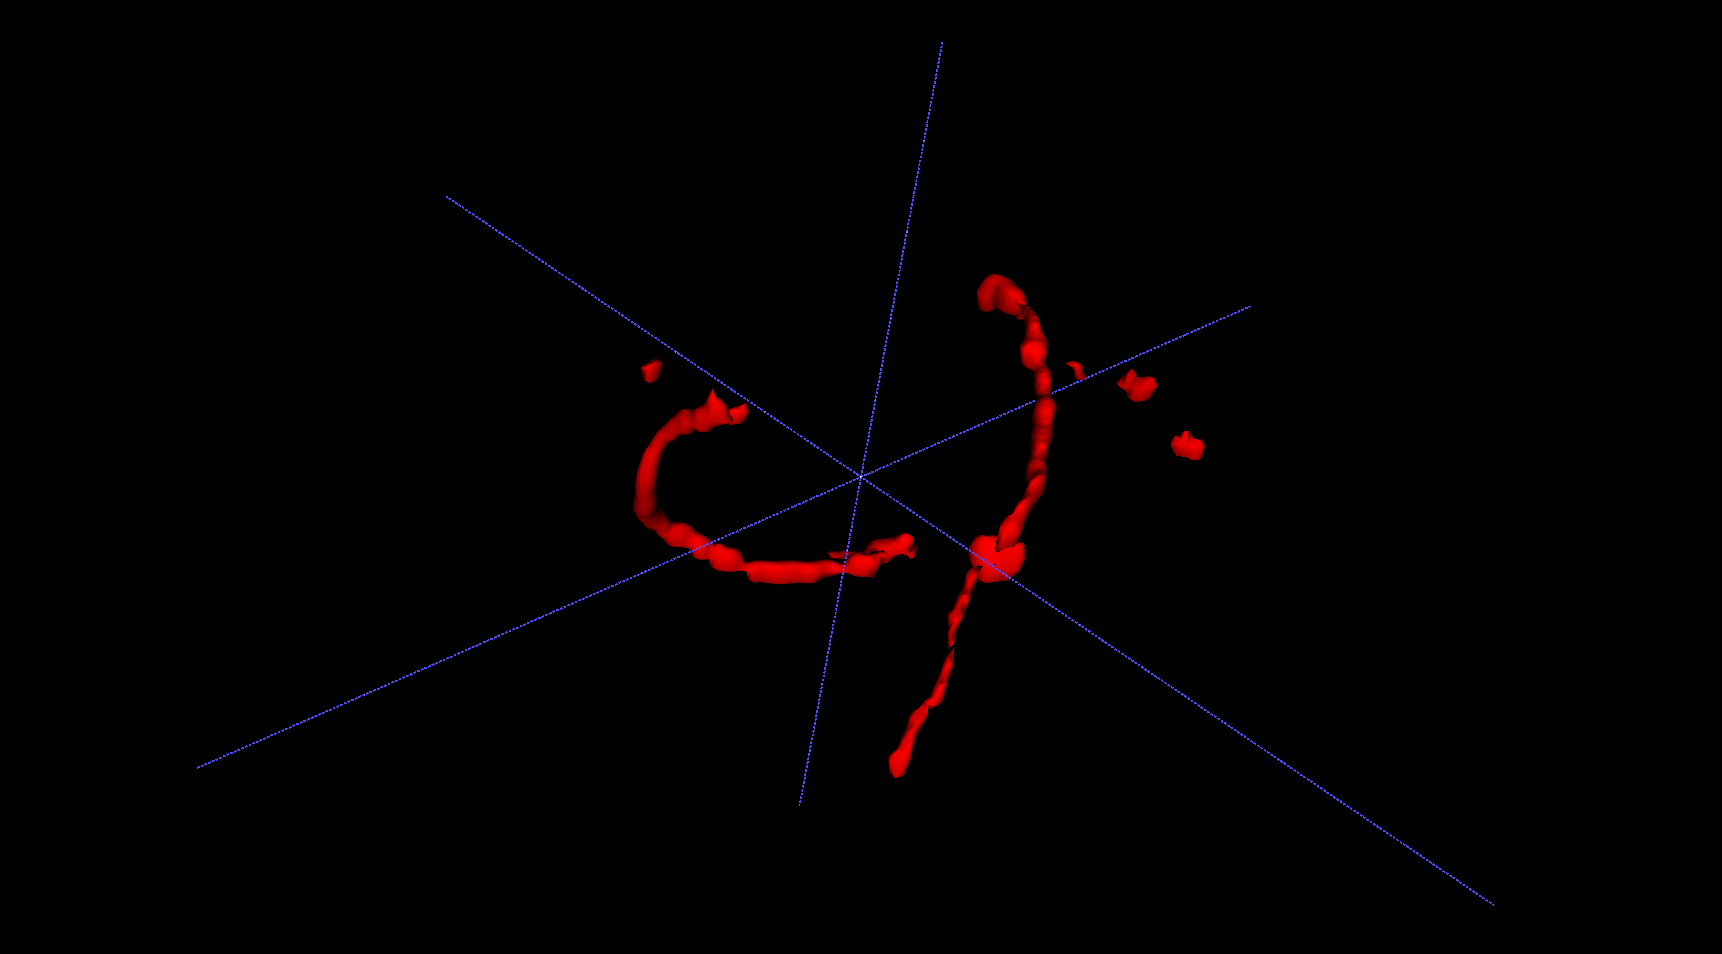
\includegraphics{fig-sample-cs-result-1-prediction}\\[3pt]
%     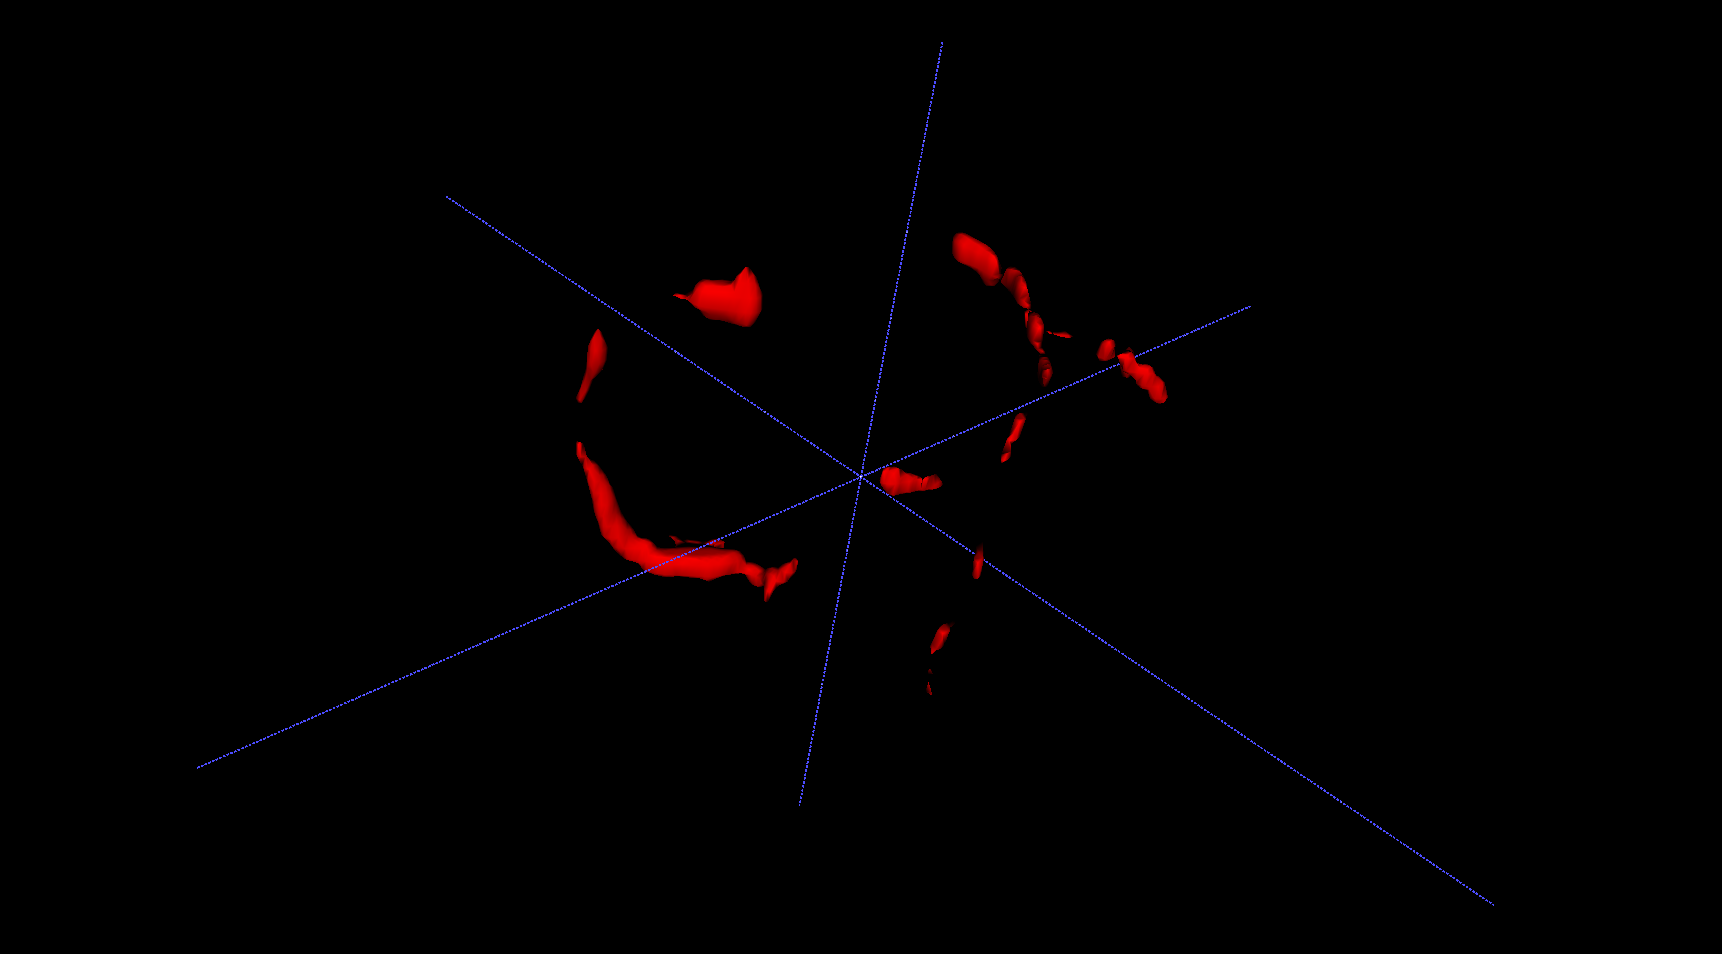
\includegraphics{fig-sample-cs-result-2-prediction}
%     \end{subfigure}
%         \caption{無顯影劑增強之電腦斷層掃描分割結果}
%     \label{fig:fig-sample-cs-result}
% \end{figure}
% 

\section{相關應用及視覺化}
本研究利用3D Slicer做為資料視覺化平台,
並將冠狀動脈分割模型、鈣化位置偵測模組以及狹窄度分析模組以3D Slicker套件的形式進行實作,
因此使用者能夠在3D Slicer的強大功能上,
使用本研究訓練完成之3D U-Net模型進行冠狀動脈分割、鈣化位置偵測與狹窄度分析。

\subsection{取得血管分析結果}
使用者可以使用3D Slicer輸入原始影像,並呼叫本研究開發之套件,將原始影像以冠狀動脈分割模型進行預測,並將分割結果輸出至3D Slicer進行視覺化。

\fig[0.75][fig:fig-3dslicer-custom-extension-example-segmentation][!hbt]{fig-3dslicer-custom-extension-example-segmentation.jpg}[本研究開發之套件介面-冠狀動脈分割][本研究開發之套件介面-冠狀動脈分割]

套件中的冠狀動脈分割功能之介面如\cref{fig:fig-3dslicer-custom-extension-example-segmentation},
使用者將原始電腦斷層影像輸入3D Slicer後,
可以在套件中選取輸入之影像,並且設定輸入影像為有顯影劑增強或是無顯影增強,
套件將會依照影像種類選擇不同的深度學習模型進行冠狀動脈分割,
另外使用者可以根據原始影像狀況,設定輸入影像欲調整至的之HU值上下界,
並利用輸出的閥值控制輸出結果,閥值愈低則分隔結果將較多,
點選執行後之結果如\cref{fig:fig-3dslicer-contrast-segmentation-result},
右上角為模型分割出之冠狀動脈以3D方式呈現之結果。
\fig[0.8][fig:fig-3dslicer-contrast-segmentation-result][!hbt]{fig-3dslicer-contrast-segmentation-result}[3D Slicer冠狀動脈分割結果視覺化][3D Slicer冠狀動脈分割結果視覺化]

\subsection{鈣化位置分析}
使用者可以設定HU值閥值以有顯影劑增強的影像進行鈣化位置分析,
套件會依照冠狀動脈分割結果、使用者指定的HU閥值、原始影像進行比對,
將冠狀動脈分割結果中,高於指定HU閥值判斷為鈣化位置,
並繪製成3D的視覺化影像,使得醫師能夠初步了解鈣化大約在冠狀動脈的哪個位置。

\fig[0.75][fig:fig-3dslicer-custom-extension-example-calcium-detection][!hbt]{fig-3dslicer-custom-extension-example-calcium-detection.jpg}[本研究開發之套件介面-鈣化位置分析][本研究開發之套件介面-鈣化位置分析]

套件中的鈣化位置分析功能之介面如\cref{fig:fig-3dslicer-custom-extension-example-calcium-detection},
使用者在以冠狀動脈分割功能得到冠狀動脈分割結果後,
可以在鈣化分析功能選取來源影像、分割結果並設定欲偵測的鈣化HU值,
點選執行後之結果如\cref{fig:fig-3dslicer-contrast-calcuim-result},
右上方的血管影像中,白色區域即為依照使用者設定所擷取出的鈣化位置。
\fig[0.8][fig:fig-3dslicer-contrast-calcuim-result][!hbt]{fig-3dslicer-contrast-calcuim-result}[3D Slicer鈣化位置視覺化][3D Slicer鈣化位置視覺化]

\subsection{狹窄度分析}
本研究開發之套件整合了3D Slicer之Extract Centerline以及Curved Planar Reformat套件,
使用者可以選取欲分析的血管開始以及結束位置,
本套件會利用Extract Centerline套件進行血管中心線擷取,
並利用Curved Planar Reformat產生以中心線拉直的血管3D圖。

\fig[0.75][fig:fig-3dslicer-custom-extension-example-stenosis-report][!hbt]{fig-3dslicer-custom-extension-example-stenosis-report.jpg}[本研究開發之套件介面-狹窄度分析][本研究開發之套件介面-狹窄度分析]

套件中的狹窄度分析功能之介面如\cref{fig:fig-3dslicer-custom-extension-example-stenosis-report},
使用者在以冠狀動脈分割功能得到冠狀動脈分割結果後,
可以選取分割結果,並設定血管開始與結束位置,
點選執行後之結果可以得到以中心線拉直的血管3D圖,
如\cref{fig:fig-3dslicer-contrast-straightened-volume},
\fig[0.75][fig:fig-3dslicer-contrast-straightened-volume][!hbt]{fig-3dslicer-contrast-straightened-volume.jpg}[冠狀動脈以中心線重組][冠狀動脈以中心線重組]
此外,本研究的套件會依照血管分割結果計算並產生血管管徑趨勢圖,
如\cref{fig:fig-3dslicer-contrast-stenosis-report}為某一受檢者的血管管徑趨勢圖,
醫師可以參考該圖片的血管管徑趨勢,輔助評估是否可能有血管狹窄的問題發生。
\fig[0.75][fig:fig-3dslicer-contrast-stenosis-report][!hbt]{fig-3dslicer-contrast-stenosis-report.jpg}[冠狀動脈血管管徑趨勢][冠狀動脈血管管徑趨勢]

本研究也利用無顯影劑資料中的分割結果較佳的RCA產生拉直之血管3D圖,
其結果如\cref{fig:fig-3dslicer-cs-straightened-volume},
顯示無顯影劑冠狀動脈分割模型所分割出的RCA也能以狹窄度分析功能獲得更進一步的利用,
增強了無顯影劑影像的利用價值。
\fig[0.75][fig:fig-3dslicer-cs-straightened-volume][!hbt]{fig-3dslicer-cs-straightened-volume.jpg}[無顯影劑影像分割之RCA以中心線重組][無顯影劑影像分割之RCA以中心線重組]

\end{document}